\clearpage
\section{Methodology and Tools}
\label{section:tools}

A large selection of methods exist to study laser-cluster interaction,
differentiating themselves through the amount of approximation taken.

Exact solution of the quantum mechanical system is, most of the time,
intractable. Theoretical investigations thus require some degree of
approximation, a compromise between feasibility and exactitude. On one end of
the spectrum, the most general methods are solving the
Time-Dependent \schrodinger Equation (TDSE) directly and Quantum Monte-Carlo
(QMC) methods. Unfortunately, these methods can only be applied to the simplest
systems of small numbers of electrons; clusters cannot be studied using these
methods.

\lrnote{few workds about the quantum monte carlo method, and a citation?}

Larger systems can be studied using \textit{ab initio} methods (``from
first principles'') which covers a wide range of techniques. In this class of
methods one can find \textit{Hartree-Fock} (HF) methods which consist on
approximating the ground state wavefunction by a single Slater determinant.
In HF methods, instantaneous electron-electron Coulomb repulsion is not
included directly in the system's Hamiltonian. Instead, only the average field
resulting from other electrons is used, giving the often used name of
\textit{self-consistent field} methods. Other \textit{ab
initio} methods are the \textit{Post Hartree-Fock} methods where electron
correlation is added. An example is the \textit{Configuration Interaction} (CI)
method. Because of their great accuracy, these methods are restricted to
relatively small systems, generally less then 10 atoms. Full \textit{ab initio}
treatment of clusters is also not possible.
\lrfatal{citations for the above}

Larger systems require
more approximations. \textit{Density Functional Theory}
is an often used method for cluster studies requiring quantum aspects, with
either quantum or semiclassical propagation. It starts by formulating an
expression for the total energy of electrons and ions and derives static and
dynamic equations from it. All approximations are done in the selection of this
(energy) functional. The upper limit on these methods is of practical reasons,
mainly computational power available. On the other side, because the chosen
functional approximate the underlying quantum system, specific quantum effects
might not be included, for example shell effects or tunnelling are neglected.
\lrfatal{citation for the above}

Because DFT methods are mean field in nature, they cannot account for the large
field fluctuations seen in strong field cluster dynamics.

Continuing on the spectrum of methods, classical methods likes Molecular
Dynamics (MD) solves Newton
equations of motion with any kind of forces between particles\cite{Skeel1998}.
When used in
laser-cluster simulations, MD generally uses the instantaneous electrostatic
(Coulomb) force between charged particles. MD codes have the advantage of being
straightforward to implement and use, give macroscopic properties easily and allow a
relatively large amount of particles to be simulated, while still allowing
specific quantum treatment when necessary (for ionization events for example). For
these reasons it is the method of choice for use in the present work.

A limitation of MD is that it cannot account for field propagation effects. For
large clusters of more than tens of thousands of atoms, these effects can become
important. PIC methods, where particles interact with a grid which propagates the
electromagnetic field (through Maxwell's equations) that other particles see
intrinsically describe these retardation effects. PIC can be successfully used
to model large clusters, but they tend to be more complex and so lack the
simplicity of MD. Additionally, because they treat particles to be of the same
size as the underlying grid, they do not describe close range interactions.
Nevertheless, Varin \textit{et al.} developed a new method that add microscopic
corrections to PIC close range interactions\cite{Varin2012}. With these microscopic
corrections, collisions between particles are described similarly to MD, insuring
that the a better description of the dynamics. This MPIC method has great prospects
as not only can it describes what MD does but can go further by including the
electromagnetic field propagation and its effects. Additionally, its scaling
allows it to describe larger clusters and it can be parallelized more easily
than MD. For smaller systems though, the complexity of PIC and MPIC and their
grid's overhead gives MD a clear advantage.

Some refinements to the MD algorithm allow it to be used for larger systems
while still keeping the same underlying code structure. For example, organizing
particles in a hierarchical tree\cite{Barnes1986,Gibbon2002} can speed up the force
calculation from a $O\pa{N^2}$ scaling to $O\pa{N \log{N}}$. More details on the
tree algorithm is presented in section \ref{section:intro:md:tree}.

On the end of the methods spectrum lies rate equations methods where a time
dependence for parameters is written down and solved. Too many approximations
are made by rate equations for use in the current work. For example, they often
assume an infinite bulk. They also cannot describe the large variation in field
and charge present in the clusters.

For a detailed review of the different methods, see Ref. \cite{Fennel2010}.

In the following section, the tools and their implementation used in the present
work will be presented. Unless stated otherwise, all implementations are original
and were done from scratch, except the Hartree-Fock-based Cowan code\cite{CowanCode} used to
in the calculation of various required cross-sections.



\subsection{Molecular Dynamics (MD)}
\label{section:tools:md}


% somewhere you should mention that the order (N^2) scaling is only for long range potentials. for short range potentials, the scaling is order (N), so we should be clear here that in this thesis, we're interested in long range (ie, coulomb)

Due to the high charge states seen in experiments with clusters the most
practical method to microscopically study the ionization dynamics is
\textit{Molecular Dynamics} (MD) methods where ions and electrons are treated
classically.

In MD, bodies interact directly through classical instantaneous forces. Even
though the method's name contains the term ``molecular'', these forces can be
of any nature; gravitational, van der Waals, Lennard-Jones, electrostatic, etc.
The method numerically integrates Newton's equations of motion, resulting in a
time evolution of the system.

The total force acting on particle $i$ of mass $m_i$ from all other $N$
particles in the system is:
\begin{align}
m_i \va_i & = \vF_i = \sum_{j \ne i} \vF_{j \rightarrow i}
\label{eqn:md:newton}
\end{align}

%
% the above is only for two-body interactions. you can do MD with more than two-body interactions - remember when we were looking at Silicon years ago, it's 3 body, for example -  so i would specifically say it's for a two-body interaction
%
In the present work, the force between charged particles is the instantaneous
electrostatic Coulomb force:
\begin{align}
\vF_{C,j \rightarrow i}\pa{\vr} & =\frac{k q_i q_j}{r_{ji}^2} \hvr_{ji}.
\label{eqn:md:coulomb:F}
\end{align}
which only depends on the distance between particles. Figure
\ref{fig:md:vectors} shows the vectors definition used throughout this work. We
define particle $i$ the particle we are interested in (for example, the
particle we are calculating the force on), and particle $j$ the particle that
is generating the field or potential that is measured at location of particle
$i$. We thus have:
\begin{align}
\vr_{j} + \vr_{j,i} & = \vr_{i} \\
\vr_{j,i} & = \vr_{i} - \vr_{j} \\
\hvr_{j,i} & = \frac{\vr_{j,i}}{\abs{\vr_{j,i}}}
\end{align}
%       _j
%       /|\
%  r_j /   \ r_ji
%     /    _\/
%    /------>i
%       r_i
%
\begin{figure}
 \centering
 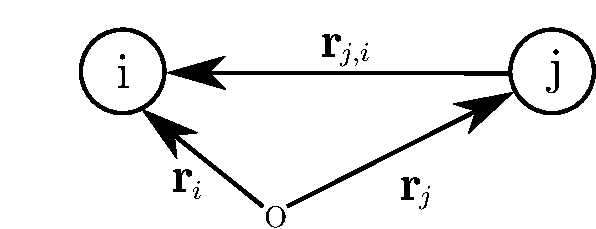
\includegraphics[width=0.5\columnwidth]{figures/vectors}
 \caption{\label{fig:md:vectors}Vectors definition between particles $i$ and $j$}
\end{figure}
%
%
Equation \eqref{eqn:md:newton} can be time integrated for every particles
$i$ using the Velocity-Verlet~(VV) scheme:
\begin{subequations}
\label{eqn:md:vv}
\begin{align}
\vx_{i}^{\pa{n+1}} & = \vx_{i}^{\pa{n}} + \vv_{i}^{\pa{n}} \Delta t +
\frac{\va_{i}^{\pa{n}}}{2} \Delta t^2, \\
\va_{i}^{\pa{n+1}} & = \frac{\vF^{\pa{n}}}{m_i} \label{eqn:md:vv:a} \\
\vv_{i}^{\pa{n+1}} & = \vv_{i}^{\pa{n}} + \frac{\va_{i}^{\pa{n}} +
\va_{i}^{\pa{n+1}}}{2} \Delta t,
\end{align}
\end{subequations}
where $\Delta t$ is the integration time step, $\vx_{i}$ the position vector,
$\vv_{i}$ the velocity vector and $\va_{i}$ the acceleration vector, all evaluated
for particle $i$ at either the time step $n$ or the next one $n+1$.
Equations \eqref{eqn:md:vv}, when applied to every 
%particles 
particle
$i$ of the system,
can thus be used to propagate in time the whole cluster. 

%Note that some
%variations of equations \eqref{eqn:md:vv} are possible but are equivalent.

%do we need the above sentence?

Every particle in the system stores its position $\vx^{\pa{n}}$, its velocity
$\vv^{\pa{n}}$ and also the total force acting on it $\vF^{\pa{n}}$. This total
force is the sum of all contribution of equation \eqref{eqn:md:coulomb:F} from
all other particles in the system.

The MD algorithm basically calculates the force between every pair of particles
in the system. Since there 
%is 
are $N$ total particles, there are
%is 
$O\pa{N^2}$
interactions to calculate. Doubling the number of particles will quadruple the
computational burden, effectively putting an upper limit on the number of
particles that can be simulated to tens of thousands.

An example cluster can be seen on figure \ref{fig:md:cluster}. 
This
%A 
cluster
is comprised
%made 
of 147 xenon atoms (large blue spheres) and absorbs some photons (red
wave-packets) from the laser field. Atoms are ionized; electron are created
(small grey spheres) which moves through the cluster. Ions are represented with
colours going from blue for neutral to red for Xe$^{5+}$. The figure was
generated using
PyMOL\footnote{\textit{The PyMOL Molecular Graphics System}, Version 1.5.0.4,
Schrödinger, LLC. \url{http://pymol.org/}} on actual simulation-created data.


\begin{figure}
 % set opaque_background, off
 \centering
 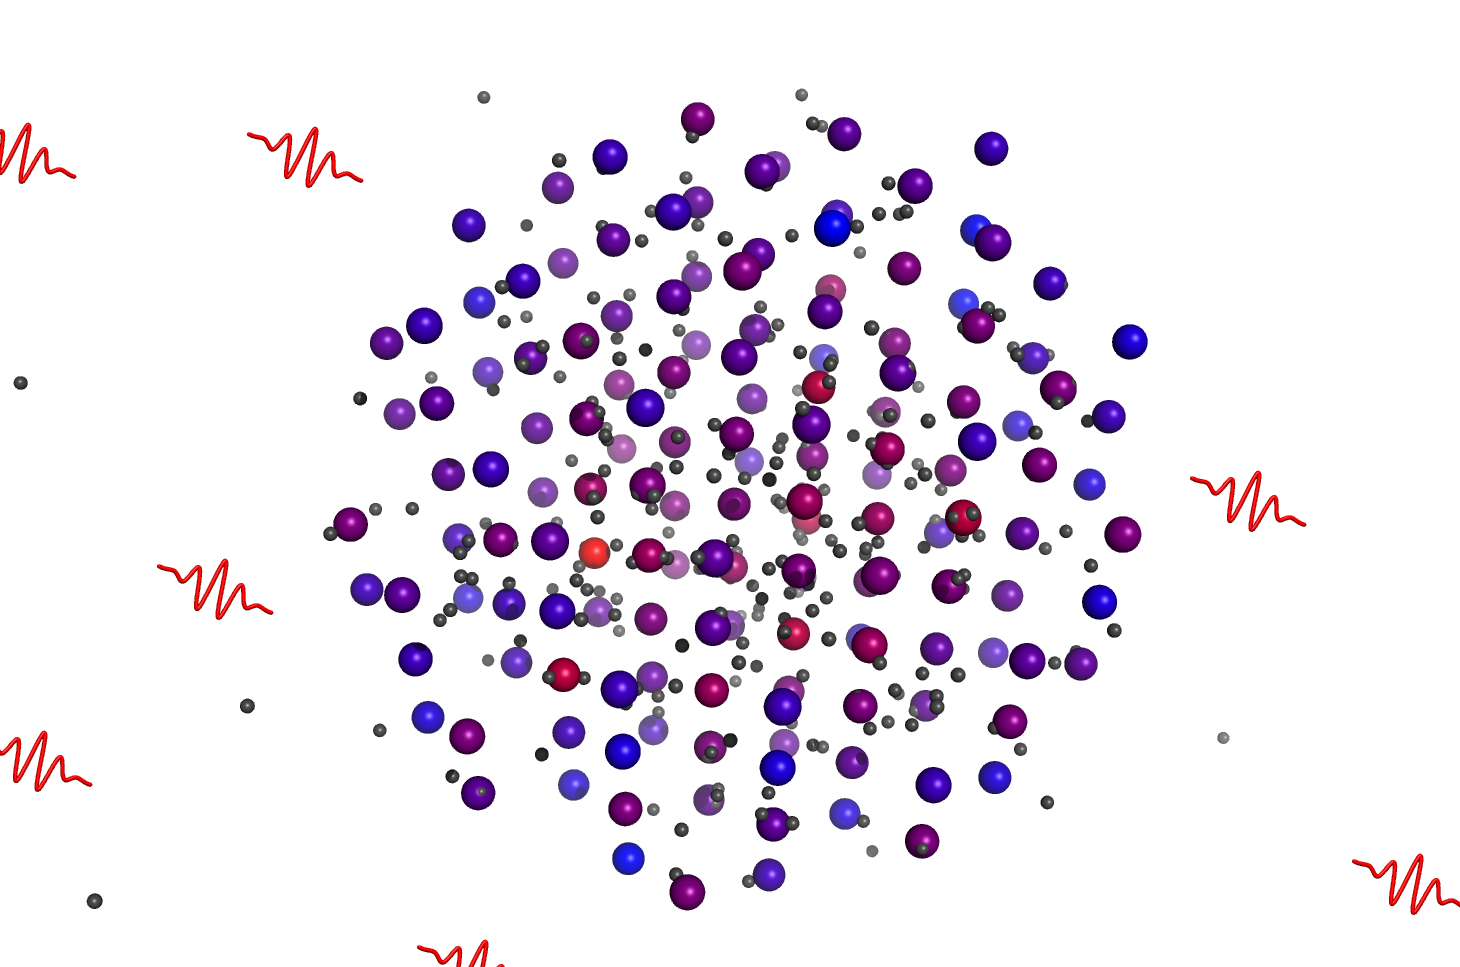
\includegraphics[width=\figurewidth]{figures/cluster}
 \caption{\label{fig:md:cluster}Example ionized Xe$_{147}$ cluster; xenon as
          large spheres with colours going from blue for neutral to full red for
          Xe$^{5+}$, electrons in small grey spheres. Photons from the laser
          field are displayed as red wave-packets.}
\end{figure}



\subsection{Short range potential shapes}
\label{section:intro:md:potentials}


%the following was changed a lot, see how you like it:

An important problem to consider is the close range behaviour 
%
of the Coulomb force 
%
in equation
\eqref{eqn:md:coulomb:F} which diverges. The problem is resolved by
changing the shape of equation \eqref{eqn:md:coulomb:F} at close range.
Different \textit{smoothing potentials} can be used to prevent the
discontinuity of the Coulomb potential (or force).

Additionally, from a quantum mechanical point-of-view, electrons should not be
able to classically recombine to an ion below the ground state energy. 
%the atomic energy level. 
A softened potential also prevents the electron from falling too deep within the potential well of an ion. If this were to happen, the cluster as a whole would become artifically heated.
However, as we will see in chapter xx, it can be important to account for the effect of a deeper potential on 
a hot electron. To
account for this, and still prevent artifical cluster heating, we have implemented electron recombination to the ground state, as described in section
\ref{section:intro:mechanisms}.

Different potential shapes were investigated for the close range potential.
Figure~\ref{fig:potential:shapes} plots the different shapes of potentials and
their respective electrostatic field. These shapes are obtained by simply
finding the location $R$ where the value and the slope of the close-range shape
$\phi_{cr}$ fits with the Coulomb potential $\phi_C$.
\begin{subequations}
\begin{align}
\left. \phi_C        \right|_{R} & = \left. \phi_{cr} \right|_{R} \\
\left. \delr{\phi_C} \right|_{R} & = \left. \delr{\phi_{cr}} \right|_{R}
\end{align}
\label{eqn:potential:to_match}
\end{subequations}

These locations $R$ are the cutoff radius of these shapes and mark the switch
between the long range Coulomb potential and the short range potential.


\subsubsection{Harmonic}

For the harmonic potential, we have:
\begin{align}
\phi_{j,H} & = -A r^2 + \phi_0
\end{align}
We note that at $r_{j,i} = 0$, the potential value is the ``potential depth''
$\phi_0$.
Matching equations \eqref{eqn:potential:to_match} at $R$ gives:
\begin{subequations}
\begin{align}
\phi_{j,H}\pa{\vr_i} & = \frac{-4 \phi_0^3}{27 \pa{k q_j}^2} r_{j,i}^2 + \phi_0
\\
R & = \frac{3 k q_j}{2 \phi_0} \\
\vE_{j,H}\pa{\vr_i} & = \frac{k q_j}{R^3} \vr_{j,i}
\end{align}
\end{subequations}


\subsubsection{Super-Gaussian}

The super-gaussian potential is given by:
\begin{align}
\phi_{j,SG}\pa{\vr_i} & = \phi_0 \ex{
                            -\frac{1}{2} \pa{\frac{r_{j,i}}{\sigma}}^{2m}
                        }
\label{eqn:potential:shapes:sg:pot}
\end{align}
In the case where $m = 1$, equation \eqref{eqn:potential:shapes:sg:pot} is simply
a gaussian shape. Matching equations~\eqref{eqn:potential:to_match} at $R$ gives
values for $\sigma$ and $R$:
\begin{subequations}
\begin{align}
\sigma  & = \frac{k q_j m^{1/2m}}{\phi_0} \ex{\frac{1}{2m}} \\
R       & = \frac{k q_j}{\phi_0} \ex{\frac{1}{2m}} \\
\vE_{j,SG} & = \frac{\phi_0 m}{r_{j,i}}
                \ex{-\frac{1}{2} \pa{\frac{r_{j,i}}{\sigma}}^{2m}}
                \pa{ \frac{r_{j,i}}{\sigma} }^{2m}
                \hvr_{j,i}
\end{align}
\label{eqn:potential:shapes:sg}
\end{subequations}





\subsubsection{Gaussian distribution}

An efficient way to correct the close range problem is to treat electrons as
charge distributions instead of point particles. There is thus no
discontinuity when the two charged distribution (particles) overlap. As such,
the electrostatic potential due to a charged particle $j$
(of gaussian shape of width $\sigma$) at location $\vr = r \hvr$ is
\begin{align}
\phi_{j}\pa{\vr} & = \frac{k q_j}{r} \erf{\frac{r}{\sigma \sqrt{2}}}
\label{eqn:md:smoothed:phi}
\end{align}
where $\erf{}$ is the error function. The associated electrostatic field is thus
\begin{align}
\vE_{j}\pa{\vr} & = -\grad{\phi_j\pa{\vr}} = k q_j \pa{
    \frac{ \erf{\frac{r}{\sigma\sqrt{2}}} }{r^2}
    - \sqrt{\frac{2}{\pi}} \frac{ \ex{-\frac{r^2}{2 \sigma^2}} }{\sigma r}
} \hvr.
\label{eqn:md:smoothed:E}
\end{align}
When the distance $r$ is large compared to $\sigma$, the error function
is tends towards 1 and the exponential tends towards 0 (since it's a gaussian
shape). The potential \eqref{eqn:md:smoothed:phi} and electric field
\eqref{eqn:md:smoothed:E} thus tend towards Coulombic for large distances.

The value of $\sigma$ is arbitrary: the smaller it is, the closer the potential
will be from the pure Coulomb one. We can set a value for $\sigma$ from the
extremum value of the potential which occurs at $\vr = 0$. At $\vr = 0$, an
indetermination $\frac{0}{0}$ occurs. Using l'Hospital rule, we get the limit
of $\phi$ as $\vr$ reaches 0:
\begin{align}
\lim_{\vr \rightarrow 0} \phi_j\pa{\vr}
    & \equiv \phi_j\pa{0} = \frac{ k q_j }{ \sigma } \sqrt{\frac{2}{\pi}}
\end{align}
from which we get the particle width:
\begin{align}
\sigma & = \frac{ k q_j }{ \phi_j\pa{0} } \sqrt{ \frac{2}{\pi}}.
\label{eqn:md:sigma}
\end{align}
The free parameter is thus the ``potential depth'' $\phi_j\pa{0}$. Even
though $\phi_j\pa{0} > 0$ we call this parameter ``depth'' since the potential
energy of an electron on top of an ion would be minimum, similar to the
gravitational potential energy of a ball is minimum at the bottom of a well.

Another problem that the smoothing of equations \eqref{eqn:md:smoothed:phi} and
\eqref{eqn:md:smoothed:E} solve is the one of \textit{numerical heating} which
occurs when particles artificially gain (or loose) energy during the
calculation of equations \eqref{eqn:md:vv}. This absence of conservation of
energy is due to a too large time step $\Delta t$. Indeed, the
discretization of equations \eqref{eqn:md:vv}, and most importantly of
subequation \eqref{eqn:md:vv:a}, assumes the force on each particle to have a
linear variation between time steps. If the time step is too large and the
curvature of equation \eqref{eqn:md:smoothed:E} cannot be sampled by the moving
particle between each time steps, then the energy will not be conserved.



Figure \ref{fig:potential:shapes} show the different potential shapes and their
respective electrostatic field.

\begin{figure}
 \centering
 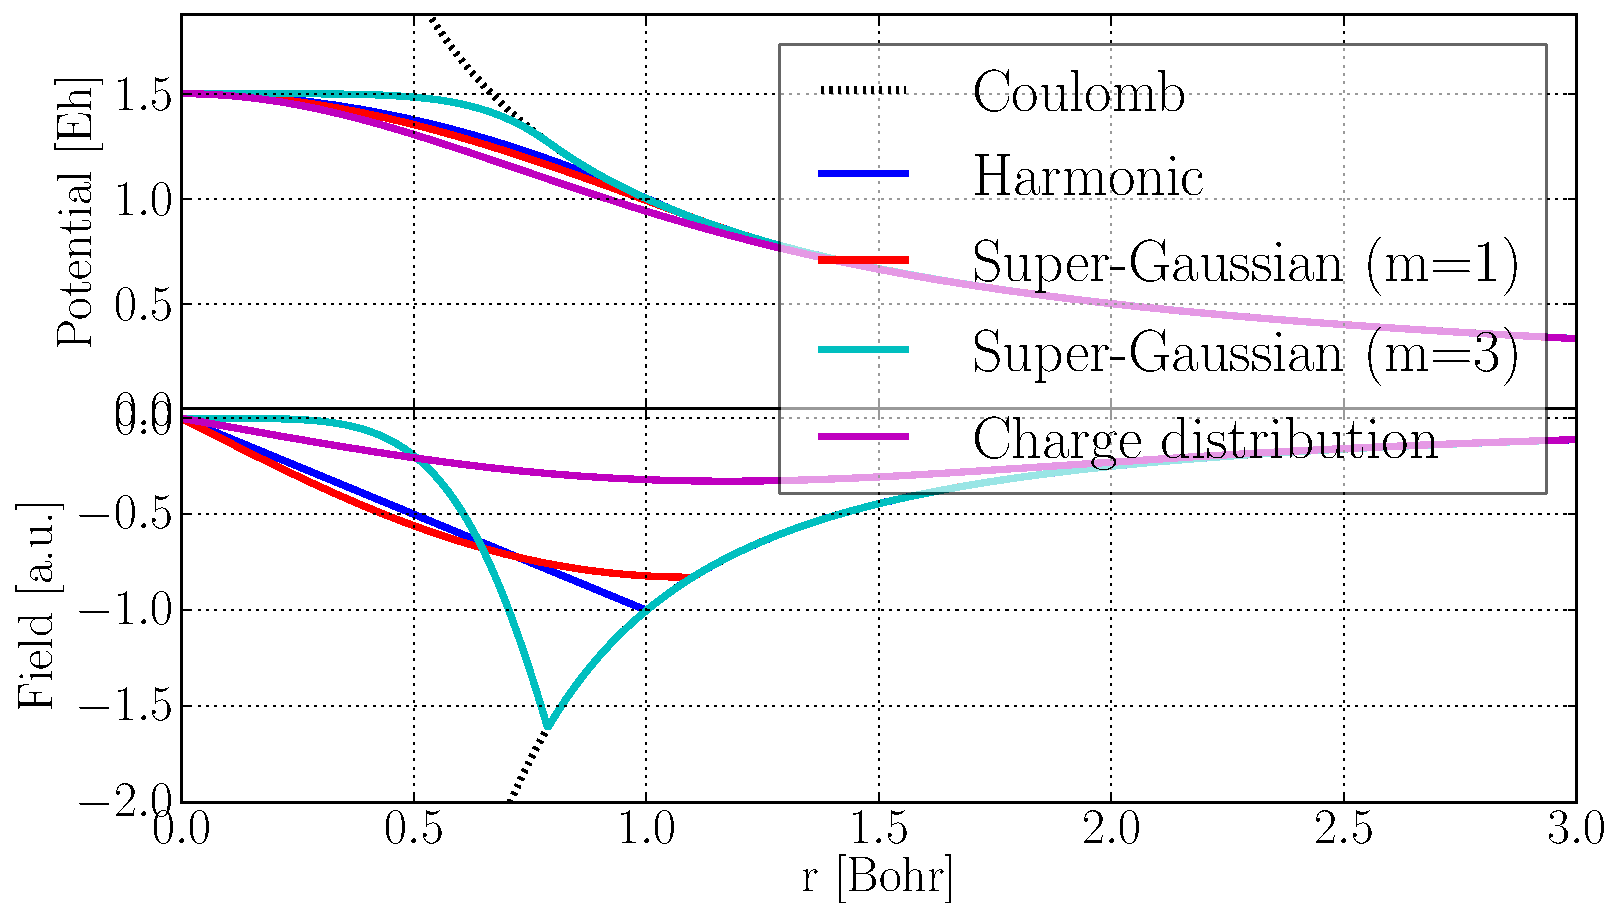
\includegraphics[width=\figurewidth]{figures/potential_shapes}
 \caption{\label{fig:potential:shapes}Potential shapes and their respective
          electric field. Note the use of atomic units and the potential depth
          $\phi_0$ = 1.5 Hartree = 40.8 eV.}
\end{figure}

It was found that the potential given by the charge distribution of equation
\eqref{eqn:md:smoothed:phi} and the associated electrostatic field of
\eqref{eqn:md:smoothed:E} give the 
%less 
least numerical heating. As explained
previously, the time discretization used to integrate the equations of motion
%assume
assumes that the change in force between two time steps is linear. As can be
seen on figure \ref{fig:potential:shapes}, the charge distribution curve
(magenta) does not have a discontinuity and is therefore the prefered one.

To validate the selection of the smoothing curve, photo-ionization was forced
on a single atom and the total energy calculated. In this ionization case, the
electron comes out of the ion with a maximum of kinetic energy so that
its total energy is the difference between the photon energy and the ionization
potential. It is thus a
good candidate %to test quantitatively measure numerical heating. 
for a quantitative measurment of numerical heating.
If the total
energy is conserved, then the selected parameters (potential depth, smoothing
curve and time step) can be used with good confidence. Figures
\ref{fig:potential:heating:dt} and \ref{fig:potential:heating:depth} show the
energy variation of the process as a function of time step (for different
potential %depth
depths) and as a function of potential depth (for different time 
%step
steps).
A time step of 0.5 attosecond is often taken as
% switched order below
it minimizes the energy variation for a large
range of potential depths, as can be seen on figure
\ref{fig:potential:heating:depth}. 
%
%Additionally, it is still above the limit where
%lowering the time step size does not reduce the error (around 0.05 as).
%
It is important to note that at around 0.05 as, there is a 
limit due to the floating point precision of the computer. The specific
parameters (time step and potential depth) are specified in the different
studies in later sections.

%can you say something about why there is a floating point precision issue? because the code is written in SI units, right? I guess this is a limitation of the code....

\begin{figure}
 \centering
 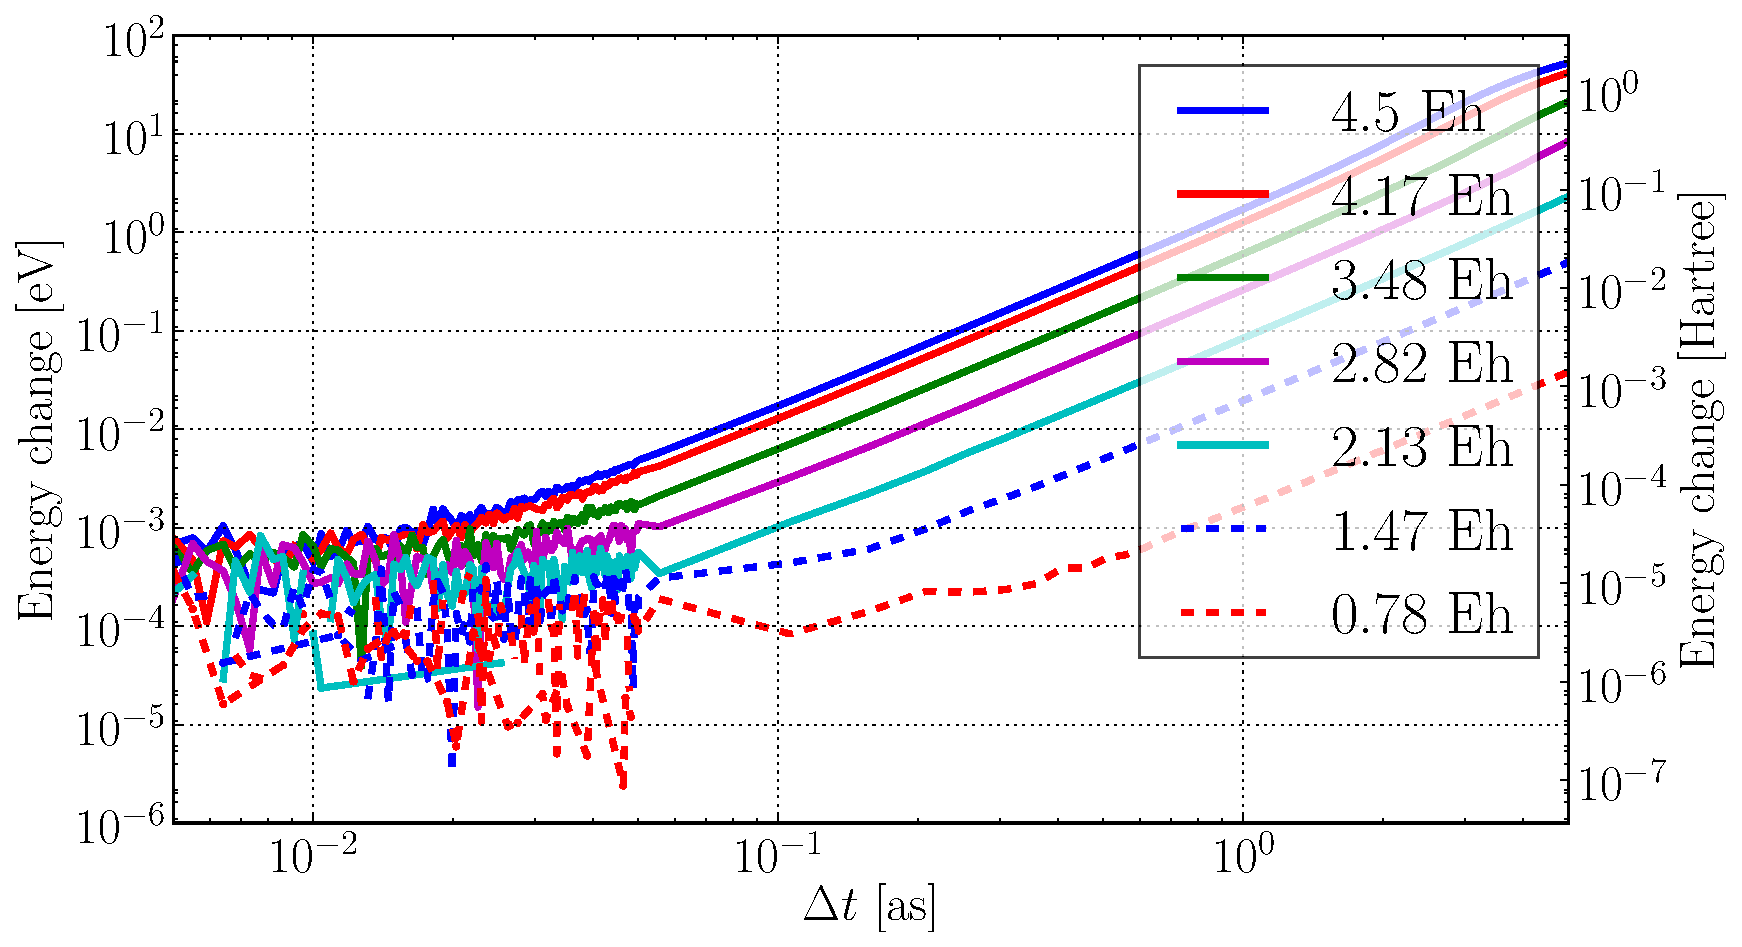
\includegraphics[width=\figurewidth]{figures/numerical_heating_dt}
 \caption{\label{fig:potential:heating:dt}Energy variation after single photon
          ionization as a function of the time step size $\Delta t$.}
\end{figure}

\begin{figure}
 \centering
 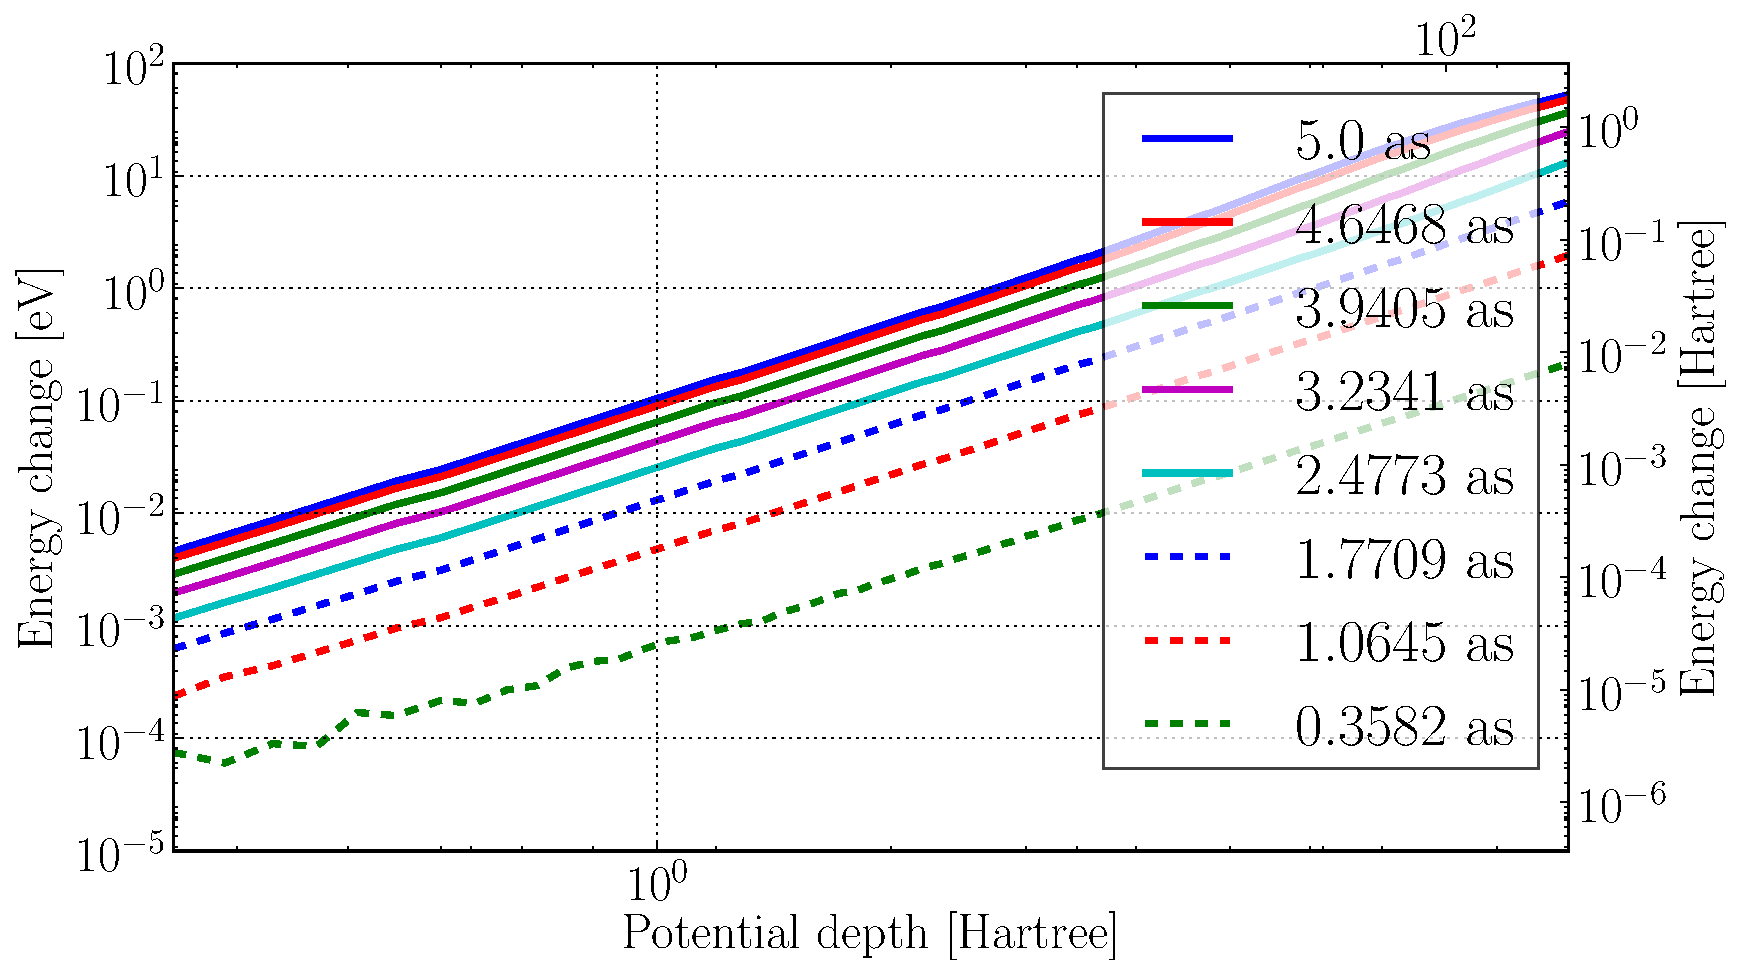
\includegraphics[width=\figurewidth]{figures/numerical_heating_D}
 \caption{\label{fig:potential:heating:depth}Energy variation after single photon
          ionization as a function of the potential depth.}
\end{figure}





\subsection{Long range potential: Hierarchical Tree algorithms}

The $O\pa{N^2}$ scaling of the MD algorithm 
%
for long-range forces
%
can be problematic when the number of
particles simulated is more than many thousands, which is a potential target
for laser-cluster interaction. Some interesting variations of the MD algorithm
exist to reduce the computational burden. 
%
One class of methods uses
\textit{hierarchical tree}
algorithms as introduced by Barnes and Hut in 1986\cite{Barnes1986}. To
reduce the computational burden, particles are grouped in a hierarchical tree
(quadtree in two dimensions, octree in three). While Barnes used his
\textit{treecode} to solve the N-body problem in the context of gravitational
interactions, it can also be applied in the electrostatic case.

The main issue with the direct calculation of forces in MD is the lack of
distinction between the close particles and distant ones. While the resulting
potential of a distant particle is small, the computational cost required to
calculate it is the same as in the case of a nearby particle. Some MD
calculations use an artificial cutoff: particles farther then this cutoff will
be ignored in the calculation of the force on one particle. This is acceptable
when the force acting on particles is short range, either due to screening or
to the nature of the force (Lennard-Jones for example).
In the present work, the dominant force is the
Coulomb force and is a long range one by nature; it thus cannot be artificially
cutoff as in the case of close range forces used in other fields.

Could distant particles be grouped together, with their contribution to the
force (or potential) being calculated only once (per ``group'')? Because
individual particles which are part of a distant group will have a similar
contribution to the potential at the location of particle $i$, the interaction
with this group can be instead approximated through the multipole
expansion\cite{Gibbon2002} of the group of particles, or cell in terms of the
tree algorithm:
\begin{align}
\phi_i & = \sum_{j~\textrm{cell}} \phi_{j \rightarrow i} = \sum_{j~{\rm cell}}
\frac{k q_j}{r_{ji}} \\
& \approx \frac{M_{c}}{R}
+ \sum_{\alpha} \frac{r_{\alpha} D_{c,\alpha}}{R^3}
+ \frac{1}{2} \sum_{\alpha,\beta} \frac{
        Q_{c,\alpha,\beta} r_{\alpha} r_{\beta}
    }{R^5}
\end{align}
where $M_{c}$, $D_{c,\alpha}$ and $Q_{c,\alpha,\beta}$ are the monopole, dipole
and quadrupole moments of the cell defined as:
\begin{subequations}
\begin{align}
M_{c}           ~~~~& = \sum_{j~\textrm{cell}} q_{j} \\
D_{c,\alpha}      ~~& = \sum_{j~\textrm{cell}} q_{j} r_{j,\alpha} \\
Q_{c,\alpha,\beta}  & = \sum_{j~\textrm{cell}} q_{j} \pa{3 r_{j,\alpha}
r_{j,\beta} - r_{j}^2} \delta_{\alpha,\beta}
\end{align}
\label{eqn:tree:moments}
\end{subequations}
and $R$ is the distance between the cell's centre-of-charge and the
particle of interest $i$.

\begin{figure}
 \centering
 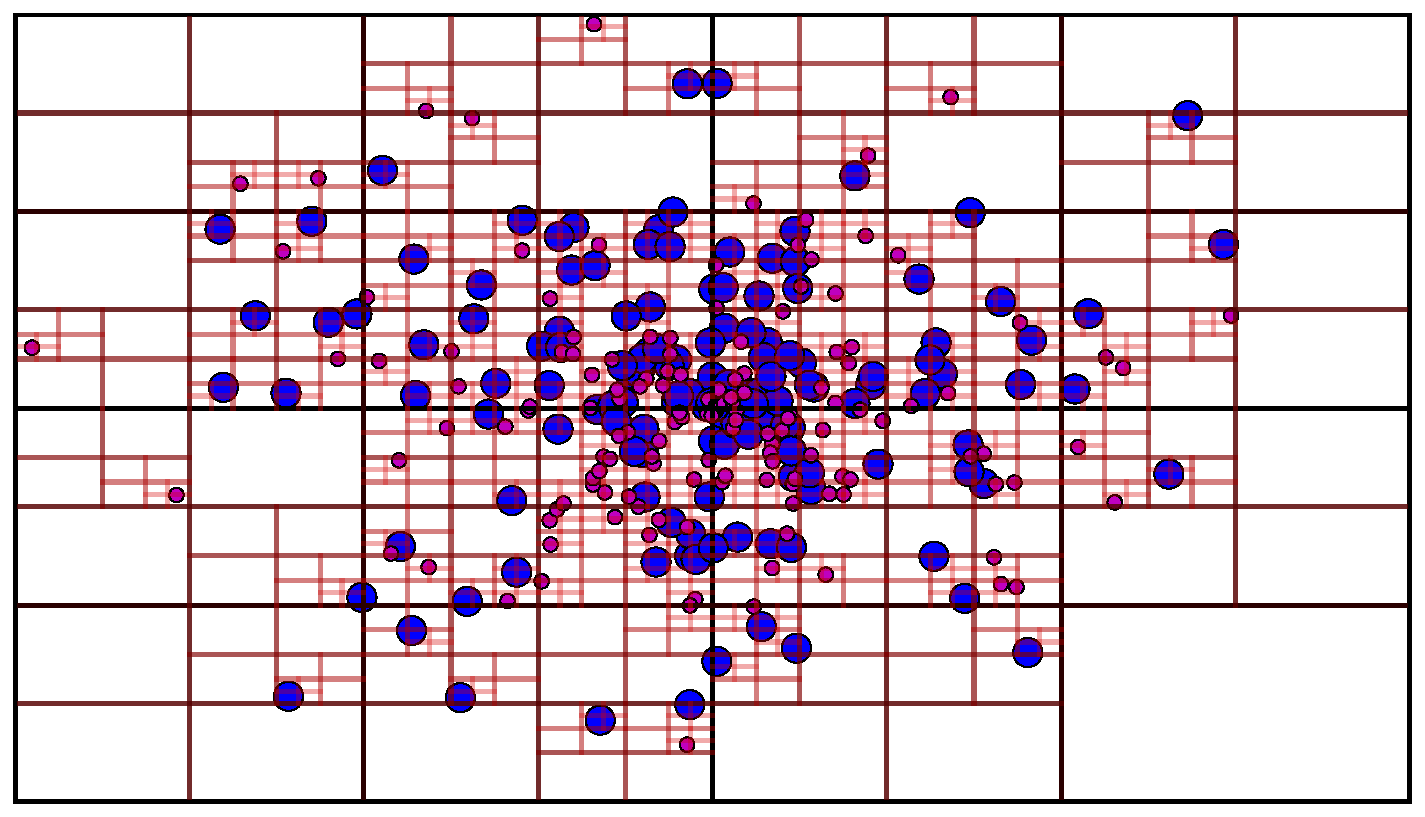
\includegraphics[width=\figurewidth]{figures/quadtree}
 \caption{\label{fig:tree:quadtree}Quadtree: 2D's equivalent of the 3D octree.
          300 particles (half ions in blue, half electrons in magenta) represent
          an exploding cluster. Cells' moments are propagated up the tree to the
          root cell. Particles far from a cell can interact directly with it
          instead of resolving all particles contained in it, thus reducing the
          computational burden.}
\end{figure}


The tree algorithm first split the computational domain into an octree (in
three dimension) or quadtree (in two dimensions) until
only a maximum of one particle is present per cell as can be seen figure
\ref{fig:tree:quadtree}. The deepest cells of the tree, containing only one particle,
are called leaves. Once every particle in the system is inserted in the tree,
the electrostatic moments are propagated from the leaves up to the root cell,
the top cell enclosing the whole domain.

Then, instead of iterating through all particles for the calculation of the
force on the particle of interest $i$, the tree is traversed. If the cell is
``far enough'' (with a given definition of far enough, discussed next) it can
be added to the a cell interaction list for later processing through the cell's
moments. In the case of
the cell being too close, it must be resolved into its  eight \textit{daughter}
cells (or four in 2D). The daughter cells containing particles are visited, while the empty
ones are ignored. The leaf cells can be reached using this process; in this
case, the particles in the leaves are considered close enough to the particle
of interest $i$ and a direct interaction is wanted. The leaf particle will thus
be added to a second interaction list containing particle-particle direct
interactions. The process is recursively repeated until all particles
are added to an interaction list, either directly or through a parent cell.
Note that an optimization done in the
implementation is to allow many particles per leaves and automatically add them
to the particles interaction list when traversing the tree, preventing trees
which are overly unbalanced.

Different selection rules exist for the criteria of ``far enough''. These
rules are called \textit{Multipole Acceptance Criteria} or
MAC\cite{Pfalzner1996}. Barnes' original one simply referred as
``\textit{s/d}'' compares an input parameter $\theta$ with the cell's size $s$
divided by the distance between the cell's center-of-charge and particle of
interest $i$ (see figure \ref{fig:tree:mac:1}).
If the ratio $s/d$ is smaller than the parameter $\theta$, the
group of particles contained inside the cell is approximated through the cell's
moments and the cell is added to the cells interaction list. At the opposite, if
the ratio is larger than $\theta$, the cell will be resolved into its daughters.
In the limit where $\theta$ reaches zero, no more cells are added to the
cells interaction list (they are all resolved) and the MD algorithm emerges, though
with a large overhead due to the tree construction and traversal.

Unfortunately, this MAC can cause huge errors when large amount of charge is
present in a corner of a cell\cite{Pfalzner1996}.
% Page 85 (97), figure 4.13
In this case, a cell could be added to the cell
interaction list even though the error introduced by the multipole expansion is
significant. Different MAC have thus been proposed to mitigate this problem.
The \textit{minimum distance} MAC replaces the distance $d$ in the MAC with the
minimum distance to one of the cell's edge (figure \ref{fig:tree:mac:2}).
The \textit{B-max} MAC instead
replaces the size of the cell with the largest distance between one of the
cell's corner to the center-of-charge (figure \ref{fig:tree:mac:3}).
Another MAC was proposed by
B\'edorf~\textit{et.~al.}~\cite{Bedorf2012} and is a mix of the two previous.
The MAC reads:
\begin{align}
d > \frac{s}{\theta} + \delta
\end{align}
where $\delta$ is the distance between the cell's geometric center and its
center-of-charge (figure \ref{fig:tree:mac:4}).
If the previous equation holds ($d$ is large enough) then the
multipole expansion is used and the cell is added to the interaction list.

\begin{figure}
 \centering
    \begin{subfigure}{0.15\columnwidth}
        \centering
        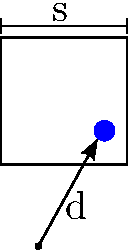
\includegraphics[width=\textwidth]{figures/mac_1}
        \caption{ $s/d$}
        \label{fig:tree:mac:1}
    \end{subfigure}
    \hspace{0.75cm}
    \begin{subfigure}{0.15\columnwidth}
        \centering
        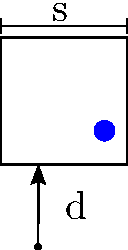
\includegraphics[width=\textwidth]{figures/mac_2}
        \caption{min. $d$}
        \label{fig:tree:mac:2}
    \end{subfigure}
    \hspace{0.75cm}
    \begin{subfigure}{0.15\columnwidth}
        \centering
        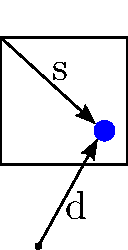
\includegraphics[width=\textwidth]{figures/mac_3}
        \caption{B-max}
        \label{fig:tree:mac:3}
    \end{subfigure}
    \hspace{0.75cm}
    \begin{subfigure}{0.15\columnwidth}
        \centering
        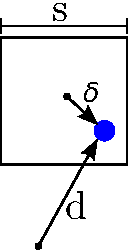
\includegraphics[width=\textwidth]{figures/mac_4}
        \caption{Bédorf\cite{Bedorf2012}}
        \label{fig:tree:mac:4}
    \end{subfigure}
\caption{Different Multipole Acceptance Criteria (MAC). See text for descriptions.}
\label{fig:tree:mac}
\end{figure}


Because not all interaction pairs are considered in the calculation of the
force and potential in this tree algorithm,
a significant speedup is obtained. Due to the tree
traversal algorithm, the scaling passes
from $O\pa{N^2}$ to $O\pa{N \log{N}}$\cite{Barnes1986,Gibbon2002,Pfalzner1996}.

A variation to the hierarchical treecode is obtained when a sufficiently large
$\theta$ is used. In this case, the root cell (the largest one) is never
resolved into its daughters. By adding more moments to the approximation then
the first three ones of equations \eqref{eqn:tree:moments} and removing
contributions of nearby particles, the \textit{Fast Multipole Method} (FMM) is
obtained\cite{Pfalzner1996}. FMM was developed by Greegard in
1988\cite{Greengard1987} independently of Barnes' hierarchical tree method.
While conceptually similar, its implementation details are quite different and
has not been implemented in the current work while the hierarchical tree
algorithm was.



\subsection{Implementation details}

\subsubsection{MD code}

Our group previously used Barnes and Hut's treecode implementation,
freely available\cite{treecode} (through the GPL version 2 license). The code was adapted
to simulate charged particles (Coulomb force) instead of masses (gravitational
force) with some ionization routines added (see for example reference
\cite{Jungreuthmayer2005}). While reducing development time by re-using already
written code, the maintenance burden introduced by many factors (initial
implementation written in the C language, usage of global variables
throughout the code, multiple coding styles from different people throughout
the years, lack of vision, lack of revision control system to give the freedom
of deleting code from the active version without loosing the ability to roll
back, many subtle and important bugs, stability issues, etc.) pushed me
to restart from scratch. This allowed using modern development techniques to be
used. For example, all development was done through a revision control system
(subversion\cite{svn} at first, then switched to git\cite{git}) in the C++
language instead of C. The object oriented nature of C++ allowed encapsulation
of different parts of the code which could then be tested and validated
individually through unit testing. This gave much better flexibility to the
code, a required asset to
push further the development of features.

A substantial number of MD packages are freely available and
their usage was considered instead of re-implementing a new one from scratch.
Examples are GROMACS\footnote{GROMACS:
\url{http://www.gromacs.org/}}, NAMD\footnote{NAMD:
\url{http://www.ks.uiuc.edu/Research/namd/}} and
LAMMPS\footnote{\url{http://lammps.sandia.gov/}}. A major issue with these
pre-existing MD packages is their target audience; they aim to simulate large
bio-molecules with mostly short range interactions. Another important problem
is the number of particles throughout the simulations; while many packages
assume a constant number of particles, the present work required creating
(ionization) and annihilating (recombination) particles throughout simulations.
Controlling the MD part of the code allowed better integration of the
ionization aspects.

Additionally, other MD packages were not mature enough or simply non-existent at the time.
For example the largely used HOOMD-blue\footnote{HOOMD-blue:
\url{http://codeblue.umich.edu/hoomd-blue/}} which uses extensively
Nvidia GPUs released its first version (v0.6.0) in February 2008.
Additionally, the knowledge and experience gained by writing from scratch such
a package is invaluable.


\subsubsection{Potential threshold $V_b$}
\label{section:intro:Vb}

Many ionization processes described previously consider an isolated atom but
clusters have close to solid density (10$^{22}$ -- 10$^{23}$ cm$^{-3}$) and
so the environment cannot be ignored.

The cluster environment can be approximated by a constant value that shifts the
potential\cite{Fennel2007}. This shift is $U_b = -e_0 V_b$ where $V_b$ is the
potential due to the cluster at the ion's location (ignoring nearby electrons)
and $U_b$ is the potential energy a test particle of charge state -1 (an electron)
would have if it was placed right on top of the ion. This can be justified by
the fact that bound states of rare gas atoms are localized close to the nucleus
and the cluster potential spatial variation around atoms is small.

To illustrate this shifting, figure \ref{fig:md:Vb} shows the potential energy
landscape of an example ``cluster'' of two ions. Plotted on this figure is the
potential energy of a test particle of charge state -1 (an electron) in the
cluster environment. The contribution from the ion is the blue dashed line on the
figure. Note the distinction between potential and potential
energy. A positive charge (an ion) creates a positive potential but the
potential \textit{energy} of the test particle (of charge state -1) in that
positive potential is negative, hence the negative curves on figure
\ref{fig:md:Vb}.



\begin{figure}
    % ./potential_landscape.py --two --ion="0,1" --ion="-15,5" --impe_r=4 \
    %     --depth=1.5 --ion_impe=0 --impe_K=0.75 --ionization --umin=-1.2 \
    %     --umax=0.3 --plot=all --rmin=-7 --rmax=7.5 --plot=U
    \begin{center}
    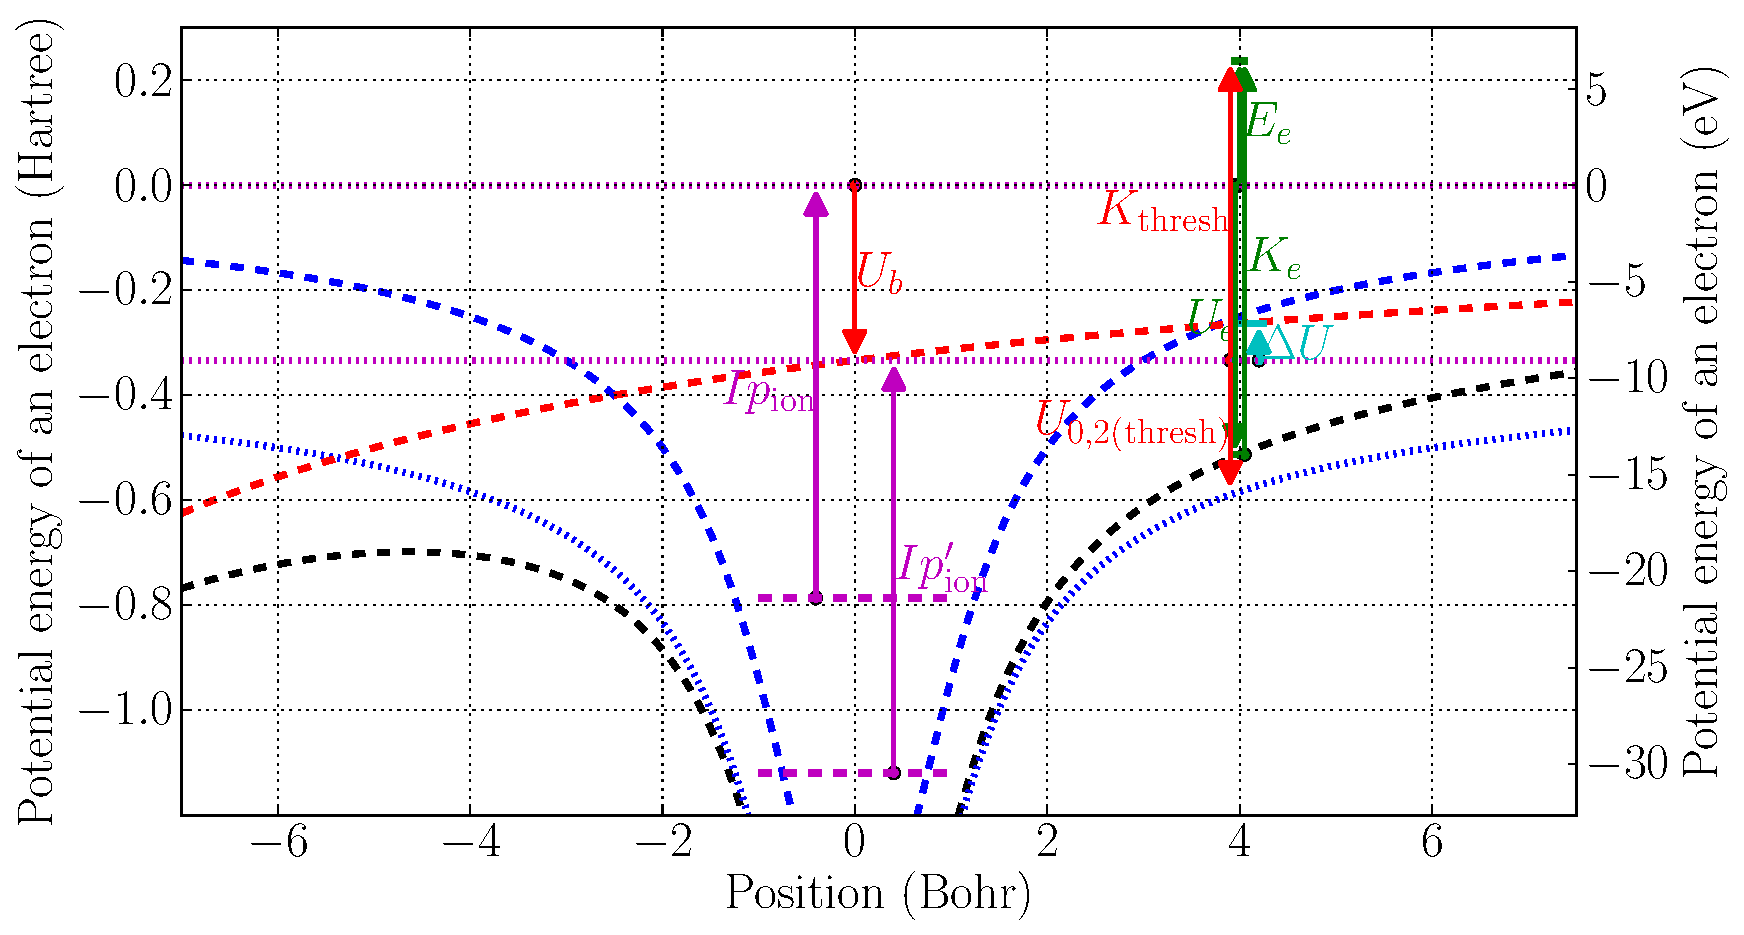
\includegraphics[width=\figurewidth]{figures/potential_landscape}
    \end{center}
    \caption{\label{fig:md:Vb}Cluster environment potential energy landscape
             and the $U_b$ approximation. A 1+ ion at $r=0$ and a 5+ at
             $r=-15$~Bohr. The potential energy curves are those of a test
             particle of charge state -1 (electron). See text for curves
             description.}
\end{figure}


Continuing in the example case of figure \ref{fig:md:Vb}, we introduce a
second ion that will simulate the cluster environment. This second ion, of
charge state 5+ and located at $r$~=~-15 Bohr, is creating a
potential that is not constant around the first ion (red-dashed line). The potential energy of
the test particle in this potential is plotted as the red dashed line. The total
potential energy of the test particle due to the two ions is plotted as a black
dashed line.

The first ion's threshold is thus influenced by the second ion. The continuum,
instead of being at zero, is shifted by $U_b$. This approximates the
influence of the second ion as being constant in the first ion's vicinity. This
threshold shift is shown on figure \ref{fig:md:Vb} as the red arrow $U_b$.

The effect of $U_b$ is to shift the ion's states to lower energies. This is
shown on the figure as Ip$_{ion}$, the energy required for a bound electron
to be promoted to the isolated ion's continuum, being shifted downward to
Ip$_{ion}'$. The effective ion's potential energy curve, also shifted by $U_b$,
is shown as the dotted blue line.

This cluster potential $U_b$ is then treated as the atom's threshold
to continuum. By using $U_b$ as the threshold, atomic properties such as
impact ionization cross-sections can be used, even in the cluster environment.



\subsubsection{Notes on ionization definition}
\label{section:intro:mechanisms:notes}

Special care needs to be taken when calculating particle energies during
ionization processes. In this work, an ionization event is defined as one
electron that leaves its parent ion, reaching infinity with a final kinetic
energy of zero.


\subsubsubsection{Single photon ionization}

In the case of single photon ionization, a new electron is created right on top
of the ion with an updated charge state. At this point, all other particles in
the cluster will not see the difference the potential created by this new
particles pair $\frac{Z+1}{r} - \frac{1}{r}$ is the same as the previous ion's
$Z/r$. For the new electron to reach infinity with a null kinetic energy, it
must have, at its creation time, enough kinetic energy to leave the ion. This
kinetic energy must thus match the potential energy between the ion (with an
updated charge state) and the electron so the total energy of the electron with
respect to the ion is zero.

Additionally, the electron will contain in its kinetic energy the difference
between the absorbed photon and the ionization potential of the ion.

\subsubsubsection{Impact ionization}

For impact ionization, the impacting electron's kinetic energy used in equation
\eqref{eqn:impact:ionization:lotz} is the kinetic energy the electron has
\textit{at infinity}, meaning that the impacting electron and the atom (or ion)
are isolated from each other.

At infinity, the electron's total energy only contains kinetic
energy. We call this kinetic energy $K_{\textrm{thresh}}$ for ``kinetic energy
above the threshold''. This $K_{\textrm{thresh}}$ can simply be calculated
as $K_{\textrm{thresh}} = \textrm{max}\pa{0, K_e + U_e}$
where $K_e$ is the
electron's kinetic energy and $U_e$ its potential energy with respect to the ion.
$K_{\textrm{thresh}}$ is thus the electron's total energy \textit{with respect
to the ion}.
In the case of a classically bound electron, the total energy is less than zero:
the max() enforces a positive kinetic energy.

When a cluster environment is present, a similar approach is taken to obtain
$K_{\textrm{thresh}}$. Instead of taking the extra energy above zero for
$K_{\textrm{thresh}}$, the extra energy above the new threshold $U_b$ is used.
This value can easily be obtained from the actual electron's kinetic energy
$K_e$, it's \textit{total} potential energy in the cluster environment and the
threshold $U_b$ by:
\begin{align}
K_{\textrm{thresh}} & = \textrm{max}\pa{0, K_e + U_e - U_b}
\label{eqn:md:kthresh}
\end{align}
and is shown on figure \ref{fig:md:Vb} as a red arrow with its base at $U_b$.


$K_{\textrm{thresh}}$ is the kinetic energy that must be used in Lotz formula
\eqref{eqn:impact:ionization:lotz}. Cross-sections are discussed in the next
section.


When an impact ionization event occurs and if the impacting electron has more kinetic
energy, it can either keep the extra, give all the extra, or give a fraction of
the extra to the new electron. We split the extra kinetic energy between the two
electrons to assure that they do not fall back unto the ion.


% Figure \ref{fig:impact:before:Z} shows the process of impact ionization when an
% electron (particle 1) of charge state -1 impacts an ion (particle 0) of charge
% state Z and creates a new electron (particle 2) right on top.
%
% \begin{figure}
%  \centering
%     \begin{subfigure}{0.48\columnwidth}
%         \centering
%         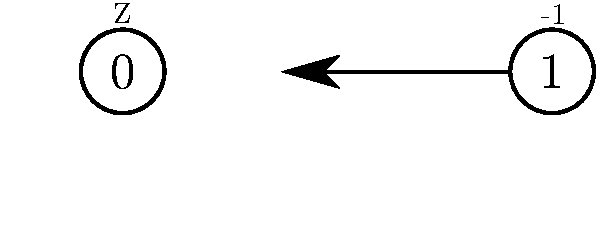
\includegraphics[width=\textwidth]{figures/impact_ionization_t00}
%         \caption{Before impact ionization (Z)}
%         \label{fig:impact:before:Z}
%     \end{subfigure}
% \\
%     \begin{subfigure}{0.48\columnwidth}
%         \centering
%         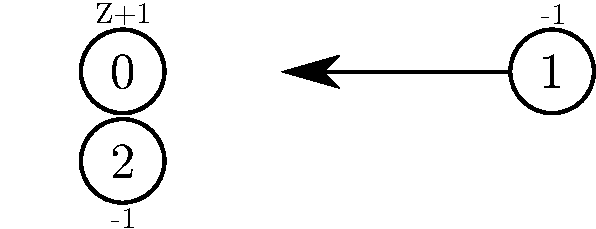
\includegraphics[width=\textwidth]{figures/impact_ionization_t0}
%         \caption{During impact ionization (Z+1)}
%         \label{fig:impact:before:Zp1}
%     \end{subfigure}
% %
%     \begin{subfigure}{0.48\columnwidth}
%         \centering
%         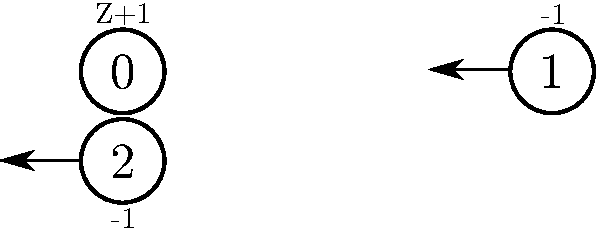
\includegraphics[width=\textwidth]{figures/impact_ionization_t1}
%         \caption{After impact ionization}
%         \label{fig:impact:after}
%     \end{subfigure}
% \caption{Impact ionization: before and after}
% \label{fig:impact:steps}
% \end{figure}


% First, let's assume the impacting electron came from infinity where it's kinetic
% energy was exactly the Ip. In that case, impact ionization will occur (considering
% its impact parameter lies inside the cross-section). By definition, we must have two
% electrons leaving to infinity: an unbound system. Such an unbound system has a total
% energy of 0.
%
% The total energy before (a) is thus:
% \begin{align}
% E^{a} & = K_{1}^{a} + U_{01}^{a} = Ip
% \label{eqn:Ea}
% \end{align}
% and after (c) ionization is:
% \begin{align}
% E^{c} & = K_{1}^{c} + K_{2}^{c} + U_{01}^{c} + U_{02}^{c} + U_{12}^{c} = 0
% \label{eqn:Ec}
% \end{align}
%
% The change in energy is thus:
% \begin{align}
% E^{a} - E^{c} & = Ip = K_{1}^{a} + U_{01}^{a} - \pa{
%     K_{1}^{c} + K_{2}^{c} + U_{01}^{c} + U_{02}^{c} + U_{12}^{c}
% }
% \end{align}
%
% The only unknown values here are $K_{1}^{c}$ and $K_{2}^{c}$ since the new electron is
% created right on top of the ion. Let's isolate the final kinetic energies:
% \begin{align}
% K_{1}^{c} + K_{2}^{c} = K_{1}^{a} + U_{01}^{a} - \pa{
%     U_{01}^{c} + U_{02}^{c} + U_{12}^{c}
% } - Ip
% \label{eqn:K1cPlusK2c}
% \end{align}
%
% We have a single constraint from equation \eqref{eqn:K1cPlusK2c} but two unknown. We thus
% give an arbitrary value to one of the two. We want the new electron to leave the ion.
% Since it is right on top of it, we can guess the required kinetic energy to be very close
% to (minus) the potential energy the electron has with respect to the ion. But this electron
% will be ``pushed'' be the impacting electron too and will thus be accelerated. To compensate
% for this push, we remove the potential energy between the two electrons from the new electron's
% kinetic energy. So the educated guess for the final kinetic energy of the new electron is:
% \begin{align}
% K_{2}^{c} & = -U_{02}^{c} - U_{12}^{c}
% \label{eqn:K2c:pushed}
% \end{align}
%
% Using equation \eqref{eqn:K2c:pushed} in equation \eqref{eqn:K1cPlusK2c} gives:
% \begin{align}
% K_{1}^{c}
%  & = K_{1}^{a} + U_{01}^{a} - \pa{
%     U_{01}^{c} + U_{02}^{c} + U_{12}^{c}
% } - Ip - K_{2}^{c} \\
%  & = K_{1}^{a} + U_{01}^{a} - \pa{
%     U_{01}^{c} + \cancel{ U_{02}^{c} } + \bcancel{ U_{12}^{c} }
% } - Ip + \cancel{ U_{02}^{c} } + \bcancel{ U_{12}^{c} } \\
% K_{1}^{c}
%  & = K_{1}^{a} + U_{01}^{a} - U_{01}^{c} - Ip
% \label{eqn:K1c:pushed}
% \end{align}
%
% The final total energy is then:
% \begin{align}
% E^{c}
%  & = \pa{
%     K_{1}^{a} + U_{01}^{a} - \cancel{ U_{01}^{c} } - Ip
%  } - \pa{
%                  \cancel{ U_{02}^{c} } + \bcancel{ U_{12}^{c} }
% } + \cancel{ U_{01}^{c} } + \cancel{ U_{02}^{c} } + \bcancel{ U_{12}^{c} } \\
%  & = K_{1}^{a} + U_{01}^{a} - Ip \\
%  & = Ip - Ip \\
% E^{c} & = 0
% \end{align}
% which is what was expected.






% Additionally, momentum is conserved by giving the two leaving electrons an angle
% of divergence. Since the impacting electron can cause ionization before being
% exactly on top of the atom or ion, the angle of divergence is given by:
%
% Figure \ref{fig:impact:direction} shows the convention of the two angles $\theta$ and $\phi$.
%
% \begin{figure}
% \begin{center}
% 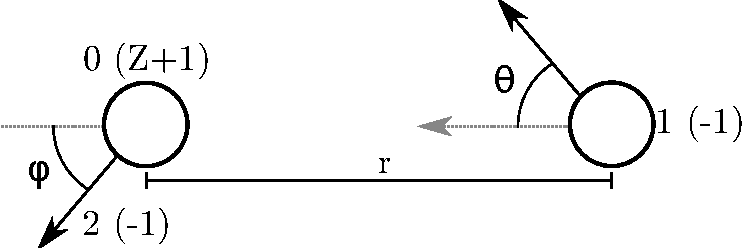
\includegraphics[width=0.8\textwidth]{figures/impact_ionization_directions}
% \end{center}
% \caption{Impact ionization: Direction for electrons}
% \label{fig:impact:direction}
% \end{figure}
%
%
% Momentum is conserved in each dimension. In this case, it's a 2-D plane.
% \begin{align}
% \vp^{a} & = \vp^{c} \\
% \vp^{a} & = m_e v_{1x}^{a} \hat{x} \\
% \vp^{c} & = m_e \pa{v_{1x}^{c} + v_{2x}^{c}} \hat{x} + m_e \pa{v_{1y}^{c} + v_{2y}^{c}} \hat{y}
% \end{align}
% with:
% \begin{subequations}
% \begin{align}
% v_{1x}^{a} & =  v_{1}^{a} \\
% v_{1x}^{c} & =  v_{1}^{c} \cosine{\theta} \\
% v_{2x}^{c} & =  v_{2}^{c} \cosine{\phi} \\
% v_{1y}^{c} & =  v_{1}^{c} \sine{\theta} \\
% v_{2y}^{c} & = -v_{2}^{c} \sine{\phi}
% \end{align}
% \end{subequations}
%
% Conservation in $x$:
% \begin{align}
% v_{1x}^{a}      & = v_{1x}^{c} + v_{2x}^{c} \\
% v_{1}^{a}       & = v_{1}^{c} \cosine{\theta} + v_{2}^{c} \cosine{\phi} \\
% \cosine{\phi}   & = \frac{v_{1}^{a} - v_{1}^{c} \cosine{\theta}}{v_{2}^{c}}
% \label{eqn:cos_phi}
% \end{align}
% and in $y$:
% \begin{align}
% 0           & = v_{1y}^{c} + v_{2y}^{c} \\
% 0           & = v_{1}^{c} \sine{\theta} - v_{2}^{c} \sine{\phi} \\
% \sine{\phi} & = \frac{v_{1}^{c}}{v_{2}^{c}} \sine{\theta}
% \label{eqn:sin_phi}
%  % \\
% % \phi        & = \asin{ \frac{v_{1}^{c}}{v_{2}^{c}} \sine{\theta} }
% \end{align}
%
% Squaring and summing \eqref{eqn:cos_phi} and \eqref{eqn:sin_phi} gives 1:
% \begin{align}
% 1
% & = \cossquared{\phi} + \sinsquared{\phi} \\
% & = \pa{ \frac{v_{1}^{a} - v_{1}^{c} \cosine{\theta}}{v_{2}^{c}} }^2
%   + \pa{ \frac{v_{1}^{c}}{v_{2}^{c}} \sine{\theta} }^{2} \\
% \pa{ v_{2}^{c} }^2
% & = \pa{ v_{1}^{a} - v_{1}^{c} \cosine{\theta} }^2
%   + \pa{ v_{1}^{c} \sine{\theta} }^{2} \\
% & = \pa{ v_{1}^{a} }^{2} + \pa{ v_{1}^{c} }^{2} \cossquared{\theta}
%     - 2 v_{1}^{a} v_{1}^{c} \cosine{\theta}
%     + \pa{ v_{1}^{c} }^{2} \sinsquared{\theta} \\
% & =   \pa{ v_{1}^{c} }^{2} \underbrace{\pa{ \cossquared{\theta} + \sinsquared{\theta} }}_{=1}
%     + \pa{ v_{1}^{a} }^{2}
%     - 2 v_{1}^{a} v_{1}^{c} \cosine{\theta} \\
% \pa{ v_{2}^{c} }^2
% & =   \pa{ v_{1}^{c} }^{2}
%     + \pa{ v_{1}^{a} }^{2}
%     - 2 v_{1}^{a} v_{1}^{c} \cosine{\theta} \\
% 2 v_{1}^{a} v_{1}^{c} \cosine{\theta}
% & =   \pa{ v_{1}^{c} }^{2}
%     + \pa{ v_{1}^{a} }^{2}
%     - \pa{ v_{2}^{c} }^2 \\
% \cosine{\theta}
% & = \frac{
%       \pa{ v_{1}^{a} }^{2}
%     + \pa{ v_{1}^{c} }^{2}
%     - \pa{ v_{2}^{c} }^2
%     }{ 2 v_{1}^{a} v_{1}^{c} }
% \label{eqn:cos_theta}
% \end{align}
%
% Equation \eqref{eqn:cos_theta} is used to get $\theta$ from $v_{1}^{a}$ (initial velocity of
% the impacting electron), $v_{1}^{c}$ (final velocity of the impacting electron) and
% $v_{2}^{c}$ (final velocity of new electron). Once the angle $\theta$ is found, $\phi$ can
% be found using \eqref{eqn:cos_phi}.
%



\subsubsection{Cross-sections}
\label{section:intro:md:cross-sections}

Implementing any kind of ionization in the model is done through cross-sections.
Because cross-sections can be obtained from experiments for any kind of target,
it is easily integrated into the model.


\subsubsubsection{Single photon ionization}

For single-photon ionization, experimental cross-sections $\sigma\pa{\omega}$
for Xenon were obtained from reference \cite{West1978} and from
reference \cite{Marr1976} for Argon.

Once cross-sections are obtained, they are converted to a rate of ionization
using
\begin{align}
\Gamma\pa{\omega} = \sigma\pa{\omega} I\pa{t}.
\label{eqn:ionization:rate:single}
\end{align}
which is equivalent to equation \eqref{eqn:ionization:rate:mpi} with $\nu = 1$.

Then, this rate is weighted\cite{Lax2006} by the time step size and compared to
a random number $r$ between 0 and 1:
\begin{align}
1 - \e{-\Gamma \Delta t} > r
\label{eqn:ionization:prob}
\end{align}
When the previous test succeeds, ionization takes place and a new electron is
created in the code.
Then, the intensity profile of the laser $I\pa{t}$ is decreased
by one photon for better description of low fluence pulses.


\subsubsubsection{Collisional processes}

For impact ionization cross-sections, Lotz formula of equation
\eqref{eqn:impact:ionization:lotz} is used with experimental parameters obtained
from reference \cite{Tawara1987} (for neutral xenon)
% Figure 254, page 317
and \cite{Heidenreich2005} (for higher charge states).
% Parameters were taken from figure 1 (a), (b) and (c)
% Note that parameters from figure 1 (a) and (b) for
% the 4+ and 5+ do not give satisfactory results. They were
% obtained by fitting the data directly from the figures
For argon, data from \cite{Lotz1967} and \cite{Lotz1970} is used.
When $K_{\textrm{thresh}} \le 0$, a null cross-section is simply used.

As for ACI, numerical cross-sections from ground state to excited state and from
excited state to continuum were calculated by Edward Ackad using a
Hartree-Fock code from Cowan\cite{Cowan1981,CowanCode}. Only the first eight excited states
were considered (with $l<4$) for charge states up to 17+ for both xenon and argon.

The impact parameter of the impacting electron is calculated by:
\begin{align}
b & = \frac{\abs{\vv \times \vr}}{\abs{\vv}}
\label{eqn:ionization:impact:parameter}
\end{align}
where $\vv$ is the impacting electron's velocity vector and $\vr$ the vector
from the impacting electron to the target. If the impacting parameter lies
inside the calculated cross section, excitation or ionization takes place. In
the case of excitation, the total cross-section of all excited states are used
and a final state randomly selected between all accessible, weighted by their
cross-sections relative to the total one.

% http://en.wikipedia.org/wiki/Neutron_cross_section#Link_to_reaction_rate_and_interpretation

\subsubsection{Recombination}

In a classical simulation electrons could cool down into the ions' infinite Coulomb
potential where they would have a total energy less then what is allowed
according to quantum mechanics. Using a smoothing potential as in equation
\eqref{eqn:md:smoothed:phi} will prevent the singularity but if the potential
depth used is deeper than the ionization potential, their can still be a problem.
Recombination is thus used to prevent such unphysical events. When an electron's
total energy (with respect to the ion) falls under the ionization potential,
recombination happens: the electron disappear from the simulation and the ion
charge state is updated.

Additionally, recombination plays an important role in the dynamics of the
exploding cluster. Experiments at FLASH in 2009 on Xenon clusters in the XUV
regime\cite{Thomas2009} could be reproduced by our models when recombination
was enable; we found that the lower charge states detected would come from the
cluster core where recombination is important. This study was published in
May 2013's edition of \textit{New Journal of Physics}\cite{Ackad2013}

Recombination was also included in the fifth study, included in section
\ref{section:papers:100nm}, as it allowed to lower the potential depth of the
ions for more physical simulations.

% Recombination is tested by calculating the total energy of an electron and
% comparing it to the threshold $U_b$ -- see figure \ref{fig:md:Vb}. If
% the energy is less then $U_b$, the electron is recombined; the ion charge is
% decremented and the electron is removed from the ion. The electron's momentum
% is transferred to the ion.\fxnote[margin,noinline]{Is the momentum really
% transferred to the ion during recomb.?}


\subsection{Quantum FDTD (QFDTD)}
\label{section:tools:qfdtd}


One model proposed to explain the high charge states seen in some experiments
is the lowering of the ionization barrier, used in conjunction with classical
MD simulations. This model assumes that an electron can be inner ionized when
the potential of a neighbouring ion lowers the potential of the electron's
parent ion. If this barrier is lowered enough so that it drops below the
electron's energy level, the electron becomes free to leave the ion and evolve
in the cluster environment. An open question is how close this model, used
with a classical MD, is to reality. Special care needs to be taken when a
particle, evolving in a quantum world, is to be treated classically. How does
the bound electron's wavefunction reacts to the presence of a second ion
perturbing the potential? How can the $U_b$ approximation to the cluster
environment, described in section \ref{section:intro:Vb}, can be tested?
Is the wavefunction really evolving into a state
where we can say the electron is shared by the two ions? If the electron is
really shared by the two ions, can we classically let it evolve inside the
cluster environment?

These questioned pushed us to look at the quantum aspects in more details. Many
different tools exist to calculate the ground state of a system, even with
multiple electrons, as describe previously. Additionally, excited states are
capital in ACI and as such we wanted a tool that could give us information not
only on the ground state but also on excited states.

After stumbling on an interesting article that used the Finite-Difference
Time-Domain (FDTD) algorithm to solve \schrodinger equation\cite{Sudiarta2007}
it was decided to explore this idea since not much work could be found on this
\textit{Quantum FDTD} (QFDTD) method and due to previous experiences
implementing electrodynamics FDTD.

FDTD is an (old) algorithm developed in 1966 by Yee\cite{Yee1966} to solve
Maxwell's equation on a grid using a leap-frog integration. The number of
scientific articles using FDTD has exponentially increased since the '80s
largely due to the increase in computation resources. Indeed, a three
dimensional grid with the three vector components of both the electric and
magnetic fields requires huge amount of memory that were definitely not present
in the late '60s. The reader is invited to read the excellent book on FDTD by
Allen Taflove and Susan Hagness\cite{Taflove2005} covering 40 years of FDTD
development in electrodynamics simulations.

Other simulation techniques like Finite-Element Methods (FEM) or Finite-Volume
Methods (FVM) can be seen as more complex then Finite-Differences Methods
(FDM). This gives some elegance and simplicity in the FDM algorithms.
Additionally, since FDTD is an explicit algorithm, implementations are
generally easy and efficient and the local nature of the algorithm makes it
easily parallelizable on distributed memory systems.

Sullivan was the first to apply the FDTD method to solve the \schrodinger
equation in his 2000 book\cite{Sullivan2000} where he obtains the wavefunction
of an electron hitting a potential barrier. Latter in 2001 he used the FDTD
method to simulate one and two electrons in a quantum dot\cite{Sullivan2001}.
The Hartree-Fock approximation was used to describe the two electrons problem
and thus required the use of Fourier transforms to calculate the Coulomb
and exchange terms. Due to this extra required calculation, the problem was
restricted to two dimensions only. The following year, he introduced a method
to calculate the eigenstates of an arbitrary system using
FDTD\cite{Sullivan2002}. This method requires two distinct simulations: the
first one finds the eigenvalues and the second one stores the states
corresponding to these eigenvalues, doubling the simulation time required.
The interaction with a magnetic field was included through the vector potential
and later\cite{Sullivan2003,Sullivan2004} used to calculate spin interaction.
Only in 2005 did the first three dimensional
simulations\cite{Sullivan2005a} were performed as proof of concept; only a
single electron was simulated. Eigenstates and eigenvalues were obtained for an
example quantum well as well as a two ions system. A more complicated three
dimensional system was later simulated in \cite{Sullivan2005b}, still with a
single electron.

Later Sudiarta suggested\cite{Sudiarta2007} a new way to use the FDTD method to
solve the \schrodinger equation for a single electron system. By switching to
\textit{imaginary time}, \schrodinger equation can be solved more easily and
more efficiently to get the eigenvalues and eigenstates of the system. It was
later shown that the interaction with a magnetic field could also be added to
the imaginary-time method\cite{Sudiarta2008} and that FDTD could be used to
construct the thermal density matrix of single particle\cite{Sudiarta2009}.

Both real-time and imaginary-time methods were implemented. Let's describe the
two algorithms.


\subsubsection{Real time}

First, let's define the time dependent \schrodinger equation describing a
wavefunction $\psi$ inside a potential $V$:
\begin{align}
\im \hbar \delt{  } \ket{\psi\pa{\vr, t}}
    & = \pa{-\frac{\hbar^2}{2 m} \laplacian{} + V\pa{\vr, t} } \ket{\psi\pa{\vr,
t}}
\label{eqn:schrodinger:si}
\end{align}
To ease the calculation, let's switch to atomic units where $\hbar = 1$, $m
= 1$ and $e_0 = 1$:
\begin{align}
\im \delt{  } \ket{\psi\pa{\vr, t}}
    & = \pa{-\frac{1}{2} \laplacian{} + V\pa{\vr, t} } \ket{\psi\pa{\vr, t}}
\label{eqn:schrodinger:au}
\end{align}
At initial time $t = 0$, the wavefunction $\ket{\psi\pa{\vr, t}}$ is
decomposed into its eigenstates basis:
\begin{align}
\ket{\psi\pa{\vr, t=0}} & = \sum_{n=0}^{\infty} c_n \ket{\phi_n\pa{\vr}}
\label{eqn:wavefunction:real:initial}
\end{align}
The time-evolution operator (or propagator) $\oU\pa{t}$ is, in atomic units:
\begin{align}
\oU\pa{t} & = \ex{ - \im t \oH }
\label{eqn:propagator:real}
\end{align}
and when applied to the initial state \eqref{eqn:wavefunction:real:initial}
gives the time evolution of the wavefunction:
\begin{align}
\oU\pa{t} \ket{\psi\pa{\vr, t=0}}
    = \ket{\psi\pa{\vr, t}}
  & = \e{ - \im t \oH } \sum_{n=0}^{\infty} c_n \ket{\phi_n\pa{\vr}}
\end{align}
Since the operator $\oH$ applied to the eigenstates
$\ket{\phi_n\pa{\vr}}$ gives the eigenvalues $E_n$, the previous equation
becomes:
\begin{align}
\ket{\psi\pa{\vr, t}}
 & = \sum_{n=0}^{\infty} \e{ - \im t E_n } c_n \ket{\phi_n\pa{\vr}}
\label{eqn:wavefunction:eigenstates:time_evolution:real}
\end{align}
The time evolution of each eigenstates is thus an oscillation between their real
and imaginary parts of which the frequency is given by the eigenvalue $E_n$.



Equation \eqref{eqn:schrodinger:au} can now be solved either in real-time or
imaginary-time, the former being explained first.

Let's separate the real and imaginary components of equation
\eqref{eqn:schrodinger:au} (and simplifying the notation):
\begin{align}
\im \delt{  } \pa{ \psi_R + \im \psi_I}
    & = \pa{-\frac{1}{2} \laplacian{} + V }
        \pa{ \psi_R + \im \psi_I} \\
\im \delt{  } \psi_R - \delt{  } \psi_I
    & = \pa{-\frac{1}{2} \laplacian{} + V } \psi_R
      + \im \pa{-\frac{1}{2} \laplacian{} + V } \psi_I
\end{align}
giving two equations describing the time evolution of two effective fields:
\begin{subequations}
\begin{align}
\delt{  } \psi_R & =   \pa{-\frac{1}{2} \laplacian{} + V } \psi_I
\label{eqn:schrodinger:real:real} \\
\delt{  } \psi_I & = - \pa{-\frac{1}{2} \laplacian{} + V } \psi_R
\label{eqn:schrodinger:real:imag}
\end{align}
\label{eqn:schrodinger:real}
\end{subequations}
The real and imaginary parts in equation \eqref{eqn:schrodinger:real} can be
compared to the electric and magnetic fields in the traditional electrodynamics
FDTD method. The integration is performed using a leap-frog scheme. We
first define $\psi_{i,j,k}^{n}$ the wavefunction located at the grid cell
$\pa{i,j,k}$ and at time step $n$. Then equation equation
\eqref{eqn:schrodinger:real:imag} is evaluated at time step $n$ and, using
(second order) central-differences, we get:
\begin{align}
\left. \delt{  } \psi_I \right|_{n}
& = \left. - \pa{-\frac{1}{2} \laplacian{} + V^{n} } \psi_R \right|_{n} \\
\frac{\psi_{I}^{n+1/2} - \psi_{I}^{n-1/2}}{\Delta t}
& = - \pa{-\frac{1}{2} \laplacian{} + V^{n} } \psi_{R}^{n} \\
\psi_{I}^{n+1/2}
& = \psi_{I}^{n-1/2} - \Delta t \pa{-\frac{1}{2} \laplacian{} + V^{n} }
\psi_{R}^{n}
\label{eqn:schrodinger:real:imag:discretized}
\end{align}
Similarly, defining the time derivative in \eqref{eqn:schrodinger:real:real} at
time step $n$ and again using (second order) central-differences:
\begin{align}
\left. \delt{  } \psi_R \right|_{n+1/2}
& = \left. \pa{-\frac{1}{2} \laplacian{} + V^{n} } \psi_I \right|_{n+1/2} \\
\frac{\psi_{R}^{n+1} - \psi_{R}^{n}}{\Delta t}
& = \pa{-\frac{1}{2} \laplacian{} + V^{n} } \psi_{I}^{n+1/2} \\
\psi_{R}^{n+1}
& = \psi_{R}^{n} + \Delta t \pa{-\frac{1}{2} \laplacian{} + V^{n} }
\psi_{I}^{n+1/2}
\label{eqn:schrodinger:real:real:discretized}
\end{align}

Lastly, the Laplacian is discretized on a grid using (second order)
central-differences:
\begin{align}
\laplacian{} \psi_{i,j,k}^{n} \approx
      \frac{ \psi_{i+1,j,k}^{n} - \psi_{i-1,j,k}^{n} }{2 \Delta x}
    + \frac{ \psi_{i,j+1,k}^{n} - \psi_{i,j-1,k}^{n} }{2 \Delta y}
    + \frac{ \psi_{i,j,k+1}^{n} - \psi_{i,j,k-1}^{n} }{2 \Delta z}
\label{eqn:laplacian:discretized}
\end{align}

Equations \eqref{eqn:schrodinger:real:imag:discretized},
\eqref{eqn:schrodinger:real:real:discretized} and
\eqref{eqn:laplacian:discretized} are then used to propagate in time the real
and imaginary components of the electronic wavefunction. Note that, contrary
to the Yee cell in the electrodynamics FDTD, the two components of the
wavefunction don't have to be defined at different location inside the grid
cell; they are defined at the same location as shown on figure
\ref{fig:qfdtd:cell}.

\begin{figure}
 \centering
    \begin{subfigure}{0.48\columnwidth}
        \centering
        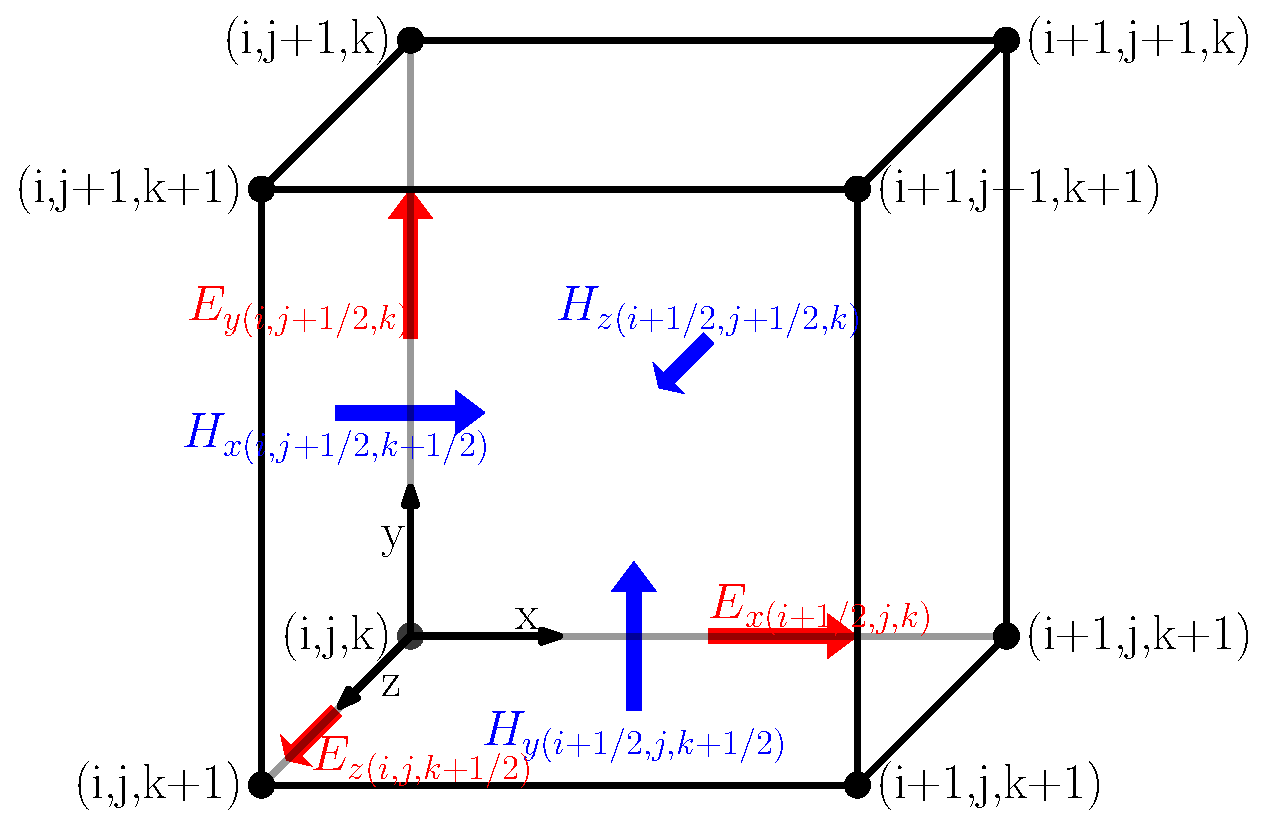
\includegraphics[width=\textwidth]{figures/fdtd_cell_yee}
        \caption{Yee cell}
        \label{fig:qfdtd:cell:yee}
    \end{subfigure}
    \begin{subfigure}{0.48\columnwidth}
        \centering
        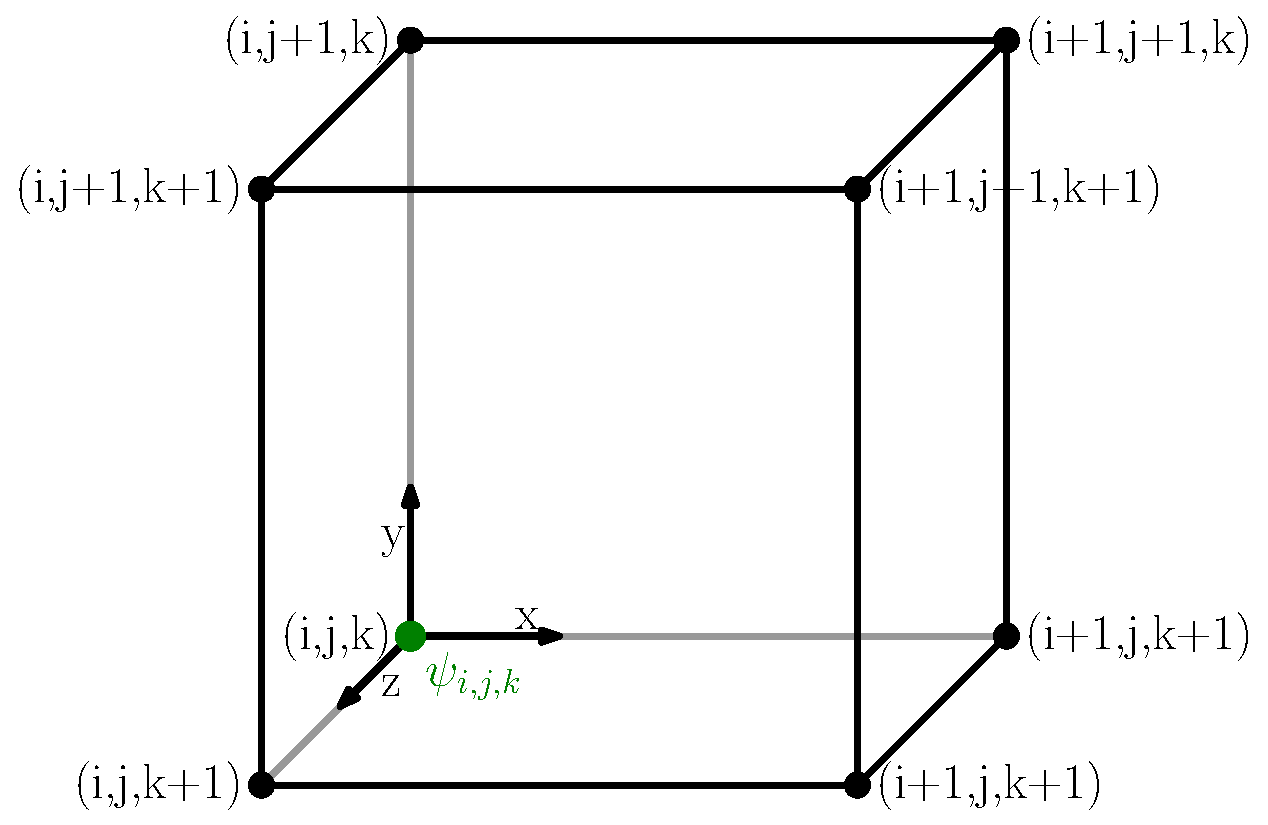
\includegraphics[width=\textwidth]{figures/fdtd_cell_qfdtd}
        \caption{QFDTD cell}
        \label{fig:qfdtd:cell:qfdtd}
    \end{subfigure}
\caption{\label{fig:qfdtd:cell}Yee cell used in electrodynamic FDTD vs QFDTD
        cell with id $\pa{i,j,k}$. Other vertices represent neighbouring cells.
        The QFDTD cell is simpler as $\psi$ is scalar (as opposed to vectorial
        electric $\vE$ and magnetic $\vH$ fields) and defined at the grid cell
        location $\pa{i,j,k}$ (compared with half-indexes shifted
        electromagnetic fields).}
\end{figure}



Equations \eqref{eqn:schrodinger:real:imag:discretized} and
\eqref{eqn:schrodinger:real:real:discretized} by themselves only describe the
time evolution of a wavefunction inside a potential; it does not give a direct
way to obtain the eigenstates of an Hamiltonian. Different approaches exist to
obtain these; Sullivan describes some of them. Eigenvalues though are
relatively easy to obtain though.

By numerically propagating in time a wavefunction $\psi$ using equations
\eqref{eqn:schrodinger:real:imag:discretized} and
\eqref{eqn:schrodinger:real:real:discretized} the system's eigenstates will
evolve according to equation
\eqref{eqn:wavefunction:eigenstates:time_evolution:real}. This evolution is an
oscillation between real and imaginary part at a specific frequency; the states'
eigenvalue. By taking a Fourier transform of the time evolution, eigenvalues
can be identified on a power spectrum. The published article of section
\ref{section:papers:qfdtd} describes a novel method of extracting the
eigenvalues of all eigenstates present in the simulated wavefunction $\psi$.



\subsubsection{Imaginary time}

The second QFDTD method, called the \textit{imaginary-time} method, differs in
that it first requires that the potential be constant in time ($V\pa{\vr, t}
\rightarrow V\pa{\vr}$). Further, a Wick rotation is performed in time ($\im t
\rightarrow \tau$) and the \schrodinger equation in imaginary time is
obtained:
\begin{align}
- \deli{}{\tau} \ket{\psi\pa{\vr, \tau}}
    & = \pa{-\frac{1}{2} \laplacian{} + V\pa{\vr} } \ket{\psi\pa{\vr, \tau}}
\label{eqn:schrodinger:imaginary}
\end{align}
Note that equation \eqref{eqn:schrodinger:imaginary} is not complex and is
similar to the heat equation.


Contrary to the real-time method, the ``time'' evolution of the imaginary
method is not oscillatory. Indeed, the propagator of equation
\eqref{eqn:propagator:real} becomes, in imaginary time:
\begin{align}
\oU\pa{\tau} & = \ex{ - \tau \oH } \label{eqn:propagator:imag}
\end{align}
and the wavefunctions evolution becomes:
\begin{align}
\ket{\psi\pa{\vr, \tau}}
 & = \sum_{n=0}^{\infty} c_n \e{ - \tau E_n } \ket{\phi_n\pa{\vr}}
\end{align}
The imaginary time evolution is thus an exponential growth with the different
eigenstates having different growth rates. It thus becomes possible to isolate
the different eigenstates from each other. A novel method to isolate these
states is described in the published article of section
\ref{section:papers:qfdtd} (page \pageref{section:papers:qfdtd}).

Because equation \eqref{eqn:schrodinger:imaginary} is real, a single scalar
field needs to be discretized on the grid. The discretization is similar to the
real-time method: equation \eqref{eqn:schrodinger:imaginary} is evaluated at
time step $n$ and the time derivative is discretized, in this case using (first
order) forward-differences (and again simplifying the notation):
\begin{align}
- \left. \deli{}{\tau} \psi \right|_{n}
    & = \cro{ \pa{-\frac{1}{2} \laplacian{} + V} \psi }_{n}
\\
\frac{\psi^{n+1} - \psi^{n}}{\Delta \tau}
    & = \pa{\frac{1}{2} \laplacian{} - V} \psi_{n}
\\
\psi^{n+1} & = \cro{1 + \Delta \tau \pa{\frac{1}{2} \laplacian{} - V}} \psi^{n}
\label{eqn:schrodinger:imaginary:discretized}
\end{align}
The Laplacian is discretized with equation \eqref{eqn:laplacian:discretized}.
Since a single scalar field is used to describe $\psi$, special care needs to
be taken in the code implementation. Indeed, equation
\eqref{eqn:schrodinger:imaginary:discretized} uses the Laplacian of the
wavefunction at the previous time step $n$ to update the wavefunction to
time step $n+1$. For example, calculating $\psi^{n+1}_{i,j,k}$ requires
$\psi^{n}_{i-1,j,k}$ and $\psi^{n}_{i+1,j,k}$ (for the $x$ derivative in the
Laplacian) but when calculating the next value in $x$ ($\psi^{n+1}_{i+1,j,k}$)
the required values are now $\psi^{n}_{i,j,k}$ and $\psi^{n}_{i+2,j,k}$, the
former being already updated. The easiest and simplest way to solve this
dependency problem is to store two grids; one for $\psi^{n}$ and another for
$\psi^{n+1}$, alternating between them when calculating equations
\eqref{eqn:schrodinger:real:imag:discretized} and
\eqref{eqn:schrodinger:real:real:discretized}.


\subsubsection{Stability criteria}

Due to the explicit nature of the FDTD algorithm (values can be obtained at the
next time step from values at the current time step only) the method is
conditionally stable; an upper bound on the time step size must be taken. The
Courant-Friedrichs-Lewy (CFL) condition gives the upper bound. Dai \textit{et
al.} derive\cite{Dai2005} the stability condition for a constant in time
potential:
\begin{align}
\Delta t < \frac{2}{
    \frac{2 \hbar}{m} \pa{
         \frac{1}{\Delta x}
        +\frac{1}{\Delta y}
        +\frac{1}{\Delta z}
        }
        + \textrm{max}\abs{V\pa{\vr}} / \hbar
    }
\end{align}



\subsubsection{Nonlinear mapping}
\label{section:tools:qfdtd:mapping}

While being simple and powerful, the QFDTD method (both real-time and
imaginary-time) suffer from a major flaw; its memory usage. Since a three
dimensional grid scales as $O\pa{N_x \cdot N_y \cdot N_z}$ where $N_i$ is the
number of grid cells in one dimension, many gigabytes of memory are often
required. Specifically in the case of QFDTD is the fact that the electronic
wavefunction must span an infinite space, or at least be truncated where
the wavefunction can be safely assumed always close to zero. Additionally,
the Coulomb potential vary drastically close to the nucleus which requires
a small grid cell size to efficiently sample, increasing uselessly the precision
far from it and multiplying the memory requirement.

A novel method was developed to concentrate three dimensional grid cells close
to centres of interest and thus reduces significantly the amount of memory
required for a given precision. Dubbed \textit{nonlinear mapping}, it maps the
discrete, integer based, space of a computer memory to the continuous regular
space. Many interesting features of this mapping make it applicable to other
type of solvers in the most generic way.

The reader will find the full details of this work in the article published
in 2011 and included in section \ref{section:papers:qfdtd}.



\subsection{Acceleration through video cards and OpenCL}
\label{section:tools:opencl}

A new trend lately in High Performance Computing (HPC) is code acceleration
through graphics cards. Similar to the ubiquitous Moore's Law in the CPU world,
video cards power evolved exponentially during the last twenty years, pushed
by the never ending need of more realistic video games. From ``dumb'' devices
drawing primitive shapes on a display, they evolved to extremely powerful
devices and started to act more like CPUs by being programmable (shaders) during
the first half 
%
decade 
% is that what you meant?
%
of 2000. The term \textit{Graphical Processing Unit} (GPU) was
coined in 1999 by Nvidia, the biggest vendor of video cards, as a selling point
to their product and to emphasize the fact that their chips were becoming more
and more %alike
like CPUs.


\subsubsection{General-Programming GPU (GP-GPU)}

Due to this increase in power, people tried to use these video cards as
accelerators for
%other things
compuations other than real video operations. Because GPUs have
intrinsically high parallelism (for example the same operation is performed on
all pixels of an image in parallel) HPC users and developers got interested.
In his 2005 book, Taflove described a way to use a video card's GPU to
accelerate his electrodynamics FDTD solver \cite{Taflove2005}. At that time no
General-Programming GPU (GP-GPU) framework existed so Taflove (and anyone
interested in using GPUs at that time) had to ``translate'' the FDTD algorithm
into one that could be understood by a video card. This process was extremely
hard as it required using low level graphic primitives; in his case, OpenGL
calls.
Normally OpenGL, the Open Graphics Library,
is used to draw animated scenes on the user's screen; it must not be confused
with OpenCL described later.
A notable example of OpenGL usage is video games where the user is immersed in a
virtual three dimensional space. The process of re-writing an algorithm into
OpenGL calls is one that only a few highly skilled and knowledgeable people can
tackle.

In 2007, Nvidia saw an opportunity for market expansion. Why not let
the non-videogames programmer use the powerful GPUs for something other than video
operations? For this to happen, a programming framework had to be released; the
number of programmers and scientists able to exploit OpenGL to their advantage
was limited. They thus released their \textit{Compute Unified Device
Architecture} (CUDA)
%, later just renamed CUDA.
CUDA allows writing normal C or
C++ programs with some extensions, called \textit{kernels}, that can be run on
the GPU. These kernels have the same structure as C functions but are executed
concurrently by every cores on the GPU\footnote{Technically, GPUs don't have
``cores'' \textit{per se} like CPUs but the comparison can still be made.}. The
number of cores on a recent consumer grade video card is now of the order of
many hundreds; a 50\$ Nvidia GT 620 has 96 CUDA cores and 1 GB of RAM, while the
GTX TITAN has 2688 CUDA cores and 6 GB but costs more than 1,000 \$. Even though
the highest priced GPU can be more expensive than complete workstations, no CPUs
can offer close to three thousand cores for a still affordable price.

A year after CUDA was released, Apple wanted a framework that would allow
programs to be accelerated on their top-of-the-line product's GPU while still
being able to run on their lower-end range of products (which did not have a
discrete video card). Additionally, some Apple products were released with ATI
video cards (Nvidia's main competitor) which, understandably, never supported
CUDA. They thus released a framework called \textit{OpenCL} (standing for
Open Compute Language) in 2008 with the help of many partners (IBM, ATI, Intel
and even Nvidia). While conceptually similar to CUDA (smaller routines are
written in a kernel function and launched individually on the GPUs by the main
program) OpenCL has the advantage of targeting heterogeneous platforms
consisting of (possibly and not limited to) many CPUs, many cores and GPUs. The
main advantage of OpenCL is its portability; a program written in OpenCL can
not only run on GPUs from ATI and Nvidia but also on traditional CPUs,
exploiting all cores available on the CPUs transparently.

It was thus decided to port the two codes (MD and QFDTD) to OpenCL to take
advantage of the GPU power while retaining portability.


\subsubsection{GPU programming challenges}

Porting a code to run on GPUs is not as simple as recompiling
for the new architecture. While being portable, OpenCL does require, unfortunately, rewriting
many parts of the code.


\subsubsubsection{Refactoring}

Some things are important to consider when porting codes to GPU frameworks.
First, because a core on a GPU is much slower than a core on a CPU,
parallelisms must be extracted from algorithms. The code must thus be
completely refactored to exploit the parallelism. For example, a CPU
implementation of the MD algorithm can be implemented by looping over particles
and calculating all properties at once, for every particle. On the contrary,
due to the high vectorized nature of GPUs, it makes more sense to calculate
only one particle property but for all particles before switching to the next
property.

Second, the main drawback of
GP-GPU programming is the fact that GPUs have their own memory, independent of
the system's memory; kernels will only have access to the device's memory. Data
required for kernel calculation must thus be first transferred to the device's
memory and similarly the resulting data must be transferred back to the host
memory where it can be further processed by the rest of the main program. Video
cards today are connected to a computer through PCI-Express (PCIe) connections.
While fast, it can still be a bottleneck if data is to be transferred back and
forth similarly to main memory. It is thus necessary to reduce to a minimum the
data transfer between the host and the device, similarly to communications in a
distributed memory parallel programming paradigm.

In the case of the MD algorithm, every interaction pair is independent of all
others and can thus be calculated concurrently; this is the basis of the
OpenCL implementation. The main loop that calculates the electrostatic field
and potential at every particle's position is implemented as an OpenCL kernel.
Each thread on the GPU will thus calculate the interaction between one particle
and all others. Once the MD kernels are launched on the GPU, they are only
halted when either ionization is to be calculated (every femtosecond) or
when data needs to be saved (to take a snapshot of the simulation for example).
This prevents the GPU from being interrupted too often and reduces the amount of
data transfers. Using this OpenCL implementation, MD simulations could be run
80 times faster than on conventional CPUs.

% 80 times faster on the GPU, right?

As for the QFDTD, only the real time algorithm was implemented as OpenCL
kernels since the imaginary time method did not require long simulation times.
As in the case of the MD, the real time algorithm is left running on the GPU
until data needs to be saved to a snapshot or post-processed to reduce
transfers.



\subsubsubsection{Debugging}

One of the most problematic part of GPU programming is the lack of debugging
tools. Many different tools and techniques exist to detect and fix problems in
normal CPU codes. The following describes them and their counterpart, when present,
on GPUs.


\subsubsubsubsection{Printing}

The simplest case of debugging is printing the variables' values to the screen
and inspecting them for
erroneous values. While not really efficient, it is sometimes useful, quick
and simple ``hack'' to get an insight of how the code is working. Unfortunately,
such printing function (such as C or C++'s \textit{printf()}) cannot be used at
all on a GPU! The reason is that the main processor must be able to
\textit{read} the variable from memory to be able to print it to screen and yet
the variable's content is \textit{not} in main memory, only the video card's
memory. It must be noted though that some OpenCL drivers (for example AMD's
APP SDK\footnote{\url{http://developer.amd.com/tools-and-sdks/heterogeneous-computing/amd-accelerated-parallel-processing-app-sdk/}}
or Intel's SDK for OpenCL Applications
2013\footnote{\url{http://software.intel.com/en-us/vcsource/tools/opencl-sdk}})
have specific extensions that allow using \textit{printf()}-like functions
inside OpenCL kernels. These extensions must explicitly be enabled in kernel
files using
\begin{verbatim}
    #pragma OPENCL EXTENSION cl_amd_printf : enable
\end{verbatim}
for the Intel SDK, or
\begin{verbatim}
    #pragma OPENCL EXTENSION cl_intel_printf : enable
\end{verbatim}
for the AMD SDK. These extensions are possible since these drivers support
running the kernels directly on the CPU. In the case of AMD, the extension only
works when the kernel are executed on the CPU (not on an AMD video card). Nvidia
does not have a similar extension for their OpenCL driver. Debugging using
printf() is thus easier when running on a CPU with either Intel's or AMD SDK.


\subsubsubsubsection{Valgrind}
\label{section:tools:opencl:valgrind}

Another useful bug squashing weapon used in debugging on Linux is called
\textit{valgrind}\footnote{\url{http://www.valgrind.org/}}. This extremely
useful tool verifies memory access and can thus report on out-of-bound accesses
(accessing memory locations which are out of range of an array), a major
type of error in programming that one \textit{has} to expect to happen.
Valgrind can also detect uses of uninitialized variables, a dangerous type of
error that can be hard to detect otherwise.

Since valgrind was specifically designed to intercept main memory access it
cannot be used when the program is running of a GPU. Alternatively, when the
program is running on the CPU through the use of the Intel or AMD SDKs, valgrind
detects a huge amount of errors, probably due to errors \textit{inside} these
SDKs, rendering the analysis useless.

One of the best tool in debugging code cannot, unfortunately, be used to debug
codes running on GPUs.


\subsubsubsubsection{Debuggers}

The last tool used in debugging is an actual debugger. A normal debugger will
take control of the program, allowing the developer to pause the execution
at any time, inspect variables' values or even change them. A popular debugger
on Linux is the free and open-source \textit{gdb}, the GNU Project
debugger\footnote{\url{https://www.gnu.org/software/gdb/}}. Many more
proprietary debuggers exist, some of them free and others expensive. Traditional
debuggers work by taking control of the program and accessing
directly their memory content. It is not possible for them to access GPU memory
or control functions inside the different SDKs. Some debuggers, like
the pricey but powerful DDT\footnote{\url{http://www.allinea.com/products/ddt/}}
allow some form of debugging capabilities on video cards. A free one
called gDEBugger\footnote{\url{http://www.gremedy.com/}} supported
debugging OpenCL kernels. It was acquired by AMD which released an updated
version\footnote{\url{http://developer.amd.com/tools-and-sdks/heterogeneous-computing/amd-gdebugger/}}
in April 2012 but discontinued it. It was superseded by
CodeXL\footnote{\url{http://developer.amd.com/tools-and-sdks/heterogeneous-computing/codexl/}}
released in February 2013. As can be seen, at the time of the code was developed
the different debuggers available were scarce, limited or expensive but are now
maturing.


\subsubsubsection{HPC Facilities}

While high performance computing (HPC) are relatively widespread and accessible,
GPU clusters are harder to find.
SHARCNET\footnote{\url{https://www.sharcnet.ca/}}, a large HPC
consortium, has two clusters containing GPUs (Angel and Monk) but they are
obviously submerged by user demand.

%\fxnote[noinline,margin]{Is the wording ok?}
%Fortunately, a grant was awarded to Professor Paul Corkum of the University of
%Ottawa by the Canada Foundation for Innovation's (CFI) Leading Edge Fund and
%New Initiatives Fund, of which a percentage was given to both Thomas Brabec
%and my supervisor Lora Ramunno for the purchase of a GPU cluster.

% how about:
My supervisor Prof. Lora Ramunno and Prof. Thomas Brabec were able to purchase
a GPU cluster, spurring the development of the GPU codes described above.

Due to my experience with GPUs, I was placed in charge of the purchase process
which consisted in building a solution that would maximize the performance
while staying under-budget, communicating with multiple vendors to validate
the solution, writing a Request for Proposals (RFP) and transparently evaluating
vendors offering. Additionally, I (remotely) installed and configured the
operating system (Gentoo Linux\footnote{\url{http://www.gentoo.org/}}) before
the equipment was shipped in August 2012 and also configured the queuing system
(Slurm\footnote{\url{http://www.schedmd.com}}) to maximize the cluster's
resources and even submitting new
features\footnote{\url{http://slurm.schedmd.com/team.html}}.

This HPC cluster (Primus), containing 20 Nvidia Tesla M2075 video cards, is an important
lab component that will be allow the research group to continue its high profile
research.


% Nic, should we move the following section forward, to where you discuss the potential shapes? I think it would make more sense there.

\subsubsection{Close-range: Look-up tables}
\label{section:intro:lut}

The preferred potential shape, the Gaussian distribution described in section
\ref{section:intro:md:potentials}, uses the error function which has a major
computational issue: it is slow, or at least too slow to be called at each interaction pair
calculation. It was decided to move to a look-up table implementation instead,
for both the CPU and GPU implementations.
The potential and field functions are pre-calculated for a charge state of 1+.
Since both potential and field are linear in charge, their value for any
particle is simply scaled by its charge state.

Once the potential and field curves are calculated, they are transferred to the
OpenCL device where they will be indexed using:
\begin{align}
x_{\textrm{norm}} & = \frac{x}{\Delta x} \\
i   & = \textrm{convert\_int\_sat\_rtz}\pa{\textrm{floor}\pa{x_{\textrm{norm}}}} \\
A   &= lut\cro{i} + \pa{lut\cro{i+1}-lut\cro{i}} \pa{x_{\textrm{norm}}-\textrm{convert\_float}\pa{i}}
\end{align}
where $x$ is the distance between the two particles, $lut$ is the array
containing the look-up table, $i$ the index of the look-up table and $A$ the
value to approximate using the look-up table. The OpenCL function
convert\_float() converts an integer to a floating point value
and convert\_int\_sat\_rtz() converts a floating point to an integer,
rounding towards zero (\_rtz) and saturating (\_sat) the conversion in case of
out-of-range
\footnote{\url{https://www.khronos.org/registry/cl/sdk/1.2/docs/man/xhtml/convert_T.html}}
(if the floating point value exceed the range of the integer type,
the maximum value for the integer is used instead of a dangerous undefined
behaviour).

This effectively does a linear interpolation between the look-up table values.
In the present work, 10,000 points are used for the table with a maximum value
for $x$ at the potential shape cutoff distance. In the case of the gaussian
distribution shape, four times the particle width $\sigma$ is used as the cutoff
distance.



\subsection{Libraries}
\label{section:tools:libraries}

Additionally to the MD and QFDTD packages, eight libraries were developed to
support some generic features shared between the two.

%\fxnote[noinline,margin]{Lora: Can I release these libraries on the internet?
%Reviewers could then see them (or use them!)}

% I don't see why not.

\subsubsection{timing.git} \label{section:tools:libraries:timing}

This library includes timing routines used to measure running time, estimated
time of arrival (ETA), code profiling, etc. It consists of 1,300 lines of C++
code and can be found here:
\url{https://gitlab.cphoton.science.uottawa.ca/nbigaouette/timing}.


\subsubsection{stdcout.git} \label{section:tools:libraries:stdcout}

Add logging features allowing saving the output of any code execution to a
(compressed or not) log file consisting of 500 lines of C++ code.
Can be found here:\\
\url{https://gitlab.cphoton.science.uottawa.ca/nbigaouette/stdcout}.


\subsubsection{prng.git} \label{section:tools:libraries:prng}

A pseudo-random number generator (PRNG) library. Wrapper around
dSFMT\cite{prng2009}, a SIMD-oriented Fast Mersenne Twister implementation.
Defines easy to use PRNG functions, distributions, seed, etc. Keeps track of
the seed and how many times pseudo-random numbers were generated, allowing
to replay the series in case of simulation reloading. 500 lines of C++ code
(not counting dSFMT) and found here:\\
\url{https://gitlab.cphoton.science.uottawa.ca/nbigaouette/prng}


\subsubsection{memory.git} \label{section:tools:libraries:memory}

Some wrappers around malloc() and calloc() that will automatically check that
memory allocation succeeded. Will also keep track of the amount of
memory allocated and allow setting a maximum value, preventing
over-allocation due to bugs or user errors. Can also return the binary
representation of a number as a string for easier debugging. 1,200 lines of
C++ code. Available here:\\
\url{https://gitlab.cphoton.science.uottawa.ca/nbigaouette/memory}


\subsubsection{io.git} \label{section:tools:libraries:io}

Input and Output library. Includes wrappers around TinyXML library\cite{tinyxml}
for reading simulation input files in XML format,
wrappers around NetCDF\cite{netcdf} for self-contained
output files, used for both post-processing and simulation snapshots.
2,950 lines of C++ code (not counting TinyXML). Available here:\\
\url{https://gitlab.cphoton.science.uottawa.ca/nbigaouette/io}


\subsubsection{libpotentials.git} \label{section:tools:libraries:libpotentials}

Functions implementing and abstracting different potential shapes as
described in section \ref{section:intro:md:potentials}. 4,300 lines of C++ code.
Available here:\\
\url{https://gitlab.cphoton.science.uottawa.ca/nbigaouette/libpotentials}


\subsubsection{oclutils.git} \label{section:tools:libraries:oclutils}

Library to ease the use of OpenCL devices. Allows listing and selecting the
best GPU available on a workstation and locking it to prevent
other simulations from using it. Contains an array abstraction to ease the
transfer of data from the host (main memory) to device (GPU memory) and
vice-versa. Also includes a SHA512 checksum check to validate memory
and detect any issue during transfers. 3,300 lines of C++ code.
Available here:
\url{https://gitlab.cphoton.science.uottawa.ca/nbigaouette/oclutils}


\subsubsection{get\_libraries.git} \label{section:tools:libraries:getlibraries}

Simple script that will download all the required libraries or
update them to the lasted version from git, compile them and install them in the
user's directory. 240 lines of bash code.
Available here:\\
\url{https://gitlab.cphoton.science.uottawa.ca/nbigaouette/get_libraries}



\subsubsection{Ionization library}
\label{section:tools:libraries:ionization}

All ionization processes described in section
\ref{section:intro:mechanisms} and consisting of 18,000 lines of C++ code.
The library is available here:\\
\url{https://gitlab.cphoton.science.uottawa.ca/nbigaouette/ionization}

The ionization library is a large part of the work as can be seen by the amount
of line of code. Each ionization processes of section
\ref{section:intro:mechanisms} have a function that, when called, will iterate
over the list of ions and calculate if the ionization takes place or not. In the
case of collisional processes (impact ionization and ACI), the iteration is over
electrons instead. The MD stores each electrons' nearest neighbour in a flag,
allowing the ionization library to calculate the required values for ionization.

To keep the library generic (so it can be used with other simulation packages,
not just the MD developed here), the library does not explicitly create
electrons (or recombine them). It instead calls functions that \textit{must}
be defined in the simulation package for the exact values to set.




